\chapter{Modelli e Strumenti}
\label{ch:modelli_strumenti}

\section{Il Modello di Task Periodico}
\label{sec:task_periodico}

\subsection{Definizioni Fondamentali}

Un \textbf{task} è una sequenza di istruzioni che, in assenza di altre attività, verrebbe eseguita dal processore in modo continuo fino al completamento. Nei sistemi Real-Time concorrenti, più task possono essere simultaneamente attivi, ma solo uno alla volta è in esecuzione. I task non in esecuzione che sono pronti a farlo vengono detti \textit{ready} e sono mantenuti in una \textbf{coda dei processi pronti} (\textit{ready queue}), gestita dalla politica di scheduling. Il meccanismo di \textbf{prelazione} (\textit{preemption}) consente al kernel di sospendere il task in esecuzione in favore di uno più urgente; il task sospeso rientra nella coda dei processi pronti. Ovviamente la parte del sistema operativo che si occupa di assegnare l'esecuzione sulle risorse disponbili è lo schedulatore, infatti  è proprio la politica scelta per lo schedulatore in fase di progettazione del sistema che impone in quale modo avviene l'esecuzione dei task nella coda dei processi pronti.

Un \textbf{task Real-Time} è un task soggetto a vincoli temporali espliciti: la robustezza del sistema dipende dal risultato dell'esecuzione del task, ma anche dall'istante in cui viene prodotto questo risultato. Per fare chiarezza Il modello formale di un task periodico $\tau_i$ è descritto nel modo seguente:

\begin{equation}
	\tau_i = (C_i,\; T_i,\; D_i)
\end{equation}


\begin{itemize}
	\item $C_i$ è il \textbf{Worst Case Execution Time} (WCET): il tempo massimo di CPU richiesto dal task in un singolo ciclo. Stimare $C_i$ non è scontato: dipende dall'architettura del processore, dalla cache, dai rami condizionali nel codice e dall'input, quindi da come viene definita la \texttt{Periodic Task} da eseguire. In questo progetto, $C_i$ viene misurato sperimentalmente tramite il sistema di tracciamento.
	\item $T_i$ è il \textbf{periodo}: l'intervallo temporale fisso tra due attivazioni consecutive. La $k$-esima istanza viene rilasciata all'istante $r_{i,k} = r_{i,0} + k \cdot T_i$.
	\item $D_i$ è la \textbf{deadline relativa}: il tempo massimo dall'istante di rilascio entro cui il task deve completare, ricordando che questo è il vincolo più importante di un sitema \texttt{Real-time}. In questo progetto si adotta il modello \textbf{implicito} ($D_i = T_i$), tipico dei sistemi di controllo in cui ogni ciclo deve terminare prima del successivo, questa scelta ovviamente se non rispettata non inificia il funzionamento del progetto è solo una scelta di progetto.
\end{itemize}

\subsection{Il Ciclo di Vita di un Task Periodico}

Il ciclo di vita di ogni istanza $k$ di $\tau_i$ si articola nelle fasi seguenti:

\begin{enumerate}
	\item \textbf{Rilascio}: al tempo $r_{i,k} = r_{i,0} + k \cdot T_i$ il task diventa pronto e viene inserito nella coda di pronto.
	\item \textbf{Attesa}: il task rimane in coda finché lo scheduler non gli assegna la CPU.
	\item \textbf{Esecuzione}: il task utilizza la CPU per un tempo $c_{i,k} \leq C_i$.
	\item \textbf{Completamento}: al tempo $f_{i,k}$, il task termina l'istanza corrente.
	\item \textbf{Sleep}: il task si sospende fino al prossimo rilascio.
\end{enumerate}

\subsection{Metriche Temporali Fondamentali}

Le metriche definite nel corso ERTS \cite{brugali_erts_2025} e misurate dal sistema sviluppato in questa tesi sono:

\begin{itemize}
	\item \textbf{Response Time}: $R_{i,k} = f_{i,k} - r_{i,k}$, differenza tra il tempo di completamento e il tempo di rilascio. Include sia il tempo di esecuzione che l'eventuale attesa in coda dovuta alla prelazione.
	
	\item \textbf{Lateness}: $L_{i,k} = f_{i,k} - d_{i,k}$, ritardo del completamento rispetto alla deadline. Se il task completa in anticipo, la lateness è negativa.
	
	\item \textbf{Laxity} (Slack Time): $X_{i,k} = d_{i,k} - r_{i,k} - C_i$, il massimo tempo per cui il task può essere ritardato dalla sua attivazione e ancora rispettare la deadline. Equivale al tempo libero residuo prima della scadenza.
	
	\item \textbf{Deadline Miss}: si verifica quando $f_{i,k} > d_{i,k}$, ovvero quando $L_{i,k} > 0$. In un sistema Hard Real-Time, ogni deadline miss è un fallimento del sistema.
	
	\item \textbf{Jitter}: variazione dell'intervallo tra attivazioni consecutive reali rispetto al periodo nominale. Il jitter assoluto è $J_{i,k} = |r_{i,k} - (r_{i,0} + k \cdot T_i)|$; il jitter relativo è la deviazione standard degli intervalli misurati. Un jitter elevato indica instabilità nella schedulazione.
	
	\item \textbf{WCET} e \textbf{ACET}: rispettivamente il massimo e la media dei tempi di esecuzione osservati su tutti i cicli registrati.
	
	\item \textbf{Utilizzazione CPU}: $U_i = C_i / T_i$ per ogni task. La somma $U = \sum_i U_i$ rappresenta la frazione di CPU complessivamente richiesta dal sistema.
\end{itemize}

\section{Schedulazione a Priorità Fissa: Rate Monotonic}
\label{sec:rms}

\subsection{Algoritmi di Scheduling Real-Time}

Il corso del prof.Brugali (ERTS \cite{brugali_erts_2025}) classifica gli algoritmi di scheduling RT in due famiglie principali:

\begin{itemize}
	\item \textbf{Algoritmi a priorità fissa}: la priorità di ogni task è assegnata staticamente e non cambia durante l'esecuzione. L'algortimo usato in questo caso è \textbf{Rate Monotonic} (RM).
	\item \textbf{Algoritmi a priorità dinamica}: la priorità cambia a runtime in base non più al periodo ma alla deadline. Il rappresentante è l'\textbf{Earliest Deadline First} (EDF), che assegna la priorità più alta al task con deadline assoluta più vicina.
\end{itemize}

In questo progetto è stato adottato Rate Monotonic, implementato tramite la policy \texttt{SCHED\_FIFO} di Linux con priorità statiche.

\subsection{Rate Monotonic: Assegnamento delle Priorità}

L'algoritmo RM, proposto da Liu e Layland nel 1973 \cite{brugali_erts_2025}, assegna staticamente a ogni task una priorità inversamente proporzionale al suo periodo: il task con periodo più breve ottiene la priorità più alta. Formalmente, per due task $\tau_i$ e $\tau_j$:

\begin{equation}
	T_i < T_j \implies P_i > P_j
\end{equation}

RM è \textbf{ottimale} nella classe degli algoritmi a priorità fissa: se un insieme di task può essere schedulato con qualsiasi algoritmo a priorità fissa, allora può essere schedulato anche con RM. Questa proprietà di ottimalità è dimostrata nel corso ERTS e costituisce la base teorica dell'assegnamento delle priorità adottato in questo progetto.


\section{POSIX e DDS per Attività Periodiche e Distribuite}
\label{sec:posix_dds}



\paragraph{Esempio senza DDS: due task su core dedicati trattato al capitolo \ref{cap:app10g_esempio}.}
Il caso più semplice è l'applicazione \texttt{app10g} (\texttt{src/app/app10g/app10g.c}): due task periodici con periodi differenti, assegnati a core fisici separati per eliminare qualsiasi contesa della CPU. Di seguito viene mostrato il main completo, che illustra l'intera sequenza di creazione dei thread Real-Time POSIX dall'inizializzazione degli attributi fino al \texttt{pthread\_join}.


\paragraph{Esempio con DDS: comunicazione distribuita trattato al capitolo \ref{cap:DDS_esempio}}
Come mostrato nelle slide ERTS \cite{brugali_erts_posix}, quando i task devono comunicare tra processi distinti su macchine diverse, la memoria condivisa non è più disponibile e si utilizza il middleware DDS. L'applicazione \texttt{Broadcastner} (\texttt{src/app/Broadcastner/Broadcastner.cpp}) mostra l'integrazione completa tra il ciclo periodico POSIX e la pubblicazione DDS: il thread \texttt{DDS\_Publish} (Core 1) esegue periodicamente la funzione \texttt{dds\_publish\_function}, mentre il thread \texttt{Activity\_1} (Core 0) simula un carico computazionale concorrente.


Il confronto tra i due esempi evidenzia le differenze architetturali introdotte dal middleware DDS:
\begin{itemize}
	\item Nel caso \texttt{app10g}, la \texttt{Periodic Task} (\texttt{activity\_load}) è ua funzione che serve per far eseguire cicli a vuoto alla CPU per simulare sforzo computazionale e  non vi è alcuna comunicazione inter-processo.
	\item Nel caso \texttt{Broadcastner}, la funzione \texttt{dds\_publish\_function} aggiunge alla computazione locale una fase di pubblicazione DDS, incapsulata tra i marker \texttt{DDS\_MSG\_START}/\texttt{END}. Il tempo tra questi due marker include la serializzazione CDR del messaggio, il trasferimento tramite SHM  o UDP e la notifica al subscriber. Questa latenza aggiuntiva è visibile nel diagramma di Gantt come un allungamento del blocco \texttt{RUN} rispetto a un task puramente computazionale con lo stesso carico \texttt{parameter}, questa differenza può essere apprezzata in modo maggiore nel capitolo dedicato al Monitor DDS di eprosima \ref{sec:monitor_dds}.
	\item la presenza del thread \texttt{Activity\_1} (Core 0, periodo 1000 ms) è presente nell' esempio \texttt{Broadcastner} per simulare un processo applicativo concorrente alla pubblicazione DDS, riproducendo uno scenario più realistico in cui il nodo publisher non ha la CPU completamente dedicata.
\end{itemize}

\clearpage
\subsection{Il Middleware DDS e la Qualità del Servizio}

Come descritto nelle slide ERTS \cite{brugali_erts_DDS}, DDS (\textit{Data Distribution Service}) è uno standard  per la comunicazione publish-subscribe anonima e decentralizzata. I principali concetti sono:

\begin{itemize}
	\item \textbf{DomainParticipant}: entità logica che partecipa a un dominio DDS. Tutti i partecipanti con lo stesso \texttt{domain\_id} possono comunicare tra loro.
	\item \textbf{Topic}: canale tipizzato identificato da un nome. Solo partecipanti che usano lo stesso topic e lo stesso tipo di messaggio possono scambiarsi dati.
	\item \textbf{DataWriter} e \textbf{DataReader}: gli oggetti concreti usati rispettivamente per pubblicare e ricevere dati.
	\item \textbf{QoS} (\textit{Quality of Service}): parametri che controllano il comportamento della comunicazione. I principali adottati in questo progetto sono:
	\begin{itemize}
		\item \textbf{Reliability}: \texttt{BEST\_EFFORT} (nessuna garanzia di consegna, minima latenza) o \texttt{RELIABLE} (consegna garantita con ritrasmissione).
		\item \textbf{Durability}: \texttt{VOLATILE} (nessuna storia salvata) o \texttt{TRANSIENT} (storia salvata in memoria locale, disponibile per subscriber che si connettono in ritardo).
		\item \textbf{Deadline}: specifica il periodo massimo tra due campioni consecutivi; se violato, il middleware notifica l'applicazione.
	\end{itemize}
\end{itemize}
\clearpage
\section{Il Monitor DDS: \textit{eProsima Fast DDS Monitor}}
\label{sec:monitor_dds}

\textbf{eProsima Fast DDS Monitor} è un'applicazione grafica open-source scaricabile a questo link: \href{https://www.eprosima.com/middleware/tools/fast-dds-monitor}{Monitor DDS}, sviluppata da eProsima che permette di osservare, in tempo reale e a posteriori, le statistiche di comunicazione di una rete DDS attiva \cite{eprosima_monitor_docs}. Si basa sul modulo statistico interno di FastDDS (\texttt{FastDDS Statistics Backend}) che, se abilitato, aggiunge automaticamente dei DataWriter interni a ogni \texttt{DomainParticipant}: questi writer pubblicano metriche di rete su topic statistici riservati (es. \texttt{HISTORY\_LATENCY\_TOPIC}, \texttt{DATA\_COUNT\_TOPIC}), che il monitor ascolta senza interferire con il traffico applicativo.

\subsection{Prerequisito: Abilitazione del Modulo Statistico}

Per far sì che i \texttt{DomainParticipant} del progetto pubblicino i propri dati statistici, è necessario abilitare il modulo statistico di FastDDS \textbf{prima}, ovvero quando si fa l'installazione sulla propria macchina del modulo fastdds e di tutte le librerie, Bisogna assicurarsi che la flag per l'installazione dei moduli statistici sia attivata. Una volta fatto nel codice l'attivazione del tracciamento avviene tramite la variabile d'ambiente \texttt{FASTDDS\_STATISTICS}:

\begin{lstlisting}[language=bash, caption={Abilitazione di tutti i topic statistici FastDDS}]
	export FASTDDS_STATISTICS="HISTORY_LATENCY_TOPIC;        \
	NETWORK_LATENCY_TOPIC;                               \
	PUBLICATION_THROUGHPUT_TOPIC;                        \
	SUBSCRIPTION_THROUGHPUT_TOPIC;                       \
	RTPS_SENT_TOPIC;RTPS_LOST_TOPIC;                     \
	DATA_COUNT_TOPIC;SAMPLE_DATAS_TOPIC;                 \
	DISCOVERY_TOPIC;PHYSICAL_DATA_TOPIC;                 \
	MONITOR_SERVICE_TOPIC"
\end{lstlisting}

Una volta settata questa variabile, ogni processo FastDDS avviato nello stesso terminale genera automaticamente i writer statistici interni. Il monitor DDS li scoprirà tramite il meccanismo di discovery e inizierà a raccogliere i dati.
\paragraph{Problema di compatibilità di versione:}
bisogna assiurarsi che la versione del monitor installata sia compatibile con la versione fastDDS presente e nel caso di mancanza di compatibilità il moitor non funziona come deve.

\subsection{Configurazione del Dominio nel Codice}

Il collegamento tra il monitor e le applicazioni del progetto dipende dal \textbf{domain ID} DDS: il monitor deve ascoltare esattamente lo stesso dominio numerico usato dai \texttt{DomainParticipant} delle applicazioni. Nel codice del progetto, il dominio viene specificato nella chiamata \texttt{start()} del wrapper \texttt{Broadcastner}:

\begin{lstlisting}[language=C++, caption={Configurazione del domain ID nella classe Broadcastner}]
	// Inizializzazione del DomainParticipant sul dominio 1.
	// Il monitor DDS deve essere configurato per ascoltare
	// esattamente questo stesso domain ID (1) per vedere
	// i DomainParticipant di questa applicazione.
	eprosima::fastdds::dds::TypeSupport msg_type(new Point_PubSubType());
	g_broadcastner.start(&msg_type, "Point", "PointTopic", 1);
	//                                                      ^
	//                                               domain_id = 1
\end{lstlisting}

Internamente, il metodo \texttt{start()} crea il \texttt{DomainParticipant} con il \texttt{domain\_id} specificato:

\begin{lstlisting}[language=C++, caption={Creazione del DomainParticipant sul dominio configurato}]
	bool Broadcastner::start(TypeSupport *msg_type,
	std::string msg_name,
	std::string topic,
	int domain_id) {
		// Il DomainParticipant viene creato sul dominio specificato.
		// Solo partecipanti con lo stesso domain_id si vedono a vicenda.
		participant_ = DomainParticipantFactory::get_instance()
		->create_participant(domain_id,
		PARTICIPANT_QOS_DEFAULT);
		// ... registrazione TypeSupport, creazione Topic e DataWriter
	}
\end{lstlisting}

Al momento di avviare il monitor, nella finestra di dialogo iniziale si deve inserire il numero \textbf{1} (o il domain ID usato dall'applicazione) per sincronizzarsi con i partecipanti corretti. Se il campo viene impostato su un dominio diverso, il monitor non vedrà nessuna entità.

\subsection{Domain View: La Mappa della Rete DDS}

La \textbf{Domain View} è la prima schermata di ispezione disponibile nel pannello principale del monitor. Visualizza un grafo che descrive la struttura fisica e logica della rete DDS attiva:

\begin{itemize}
	\item \textbf{Struttura gerarchica fisica}: ogni \textit{Host} (macchina fisica) contiene uno o più \textit{User} (utenti di sistema), che a loro volta contengono i \textit{Process} (processi in esecuzione). Questa gerarchia è resa possibile dall'attivazione del topic \texttt{PHYSICAL\_DATA\_TOPIC} nella variabile d'ambiente.
	
	
	\begin{figure}[htbp]
		\centering
		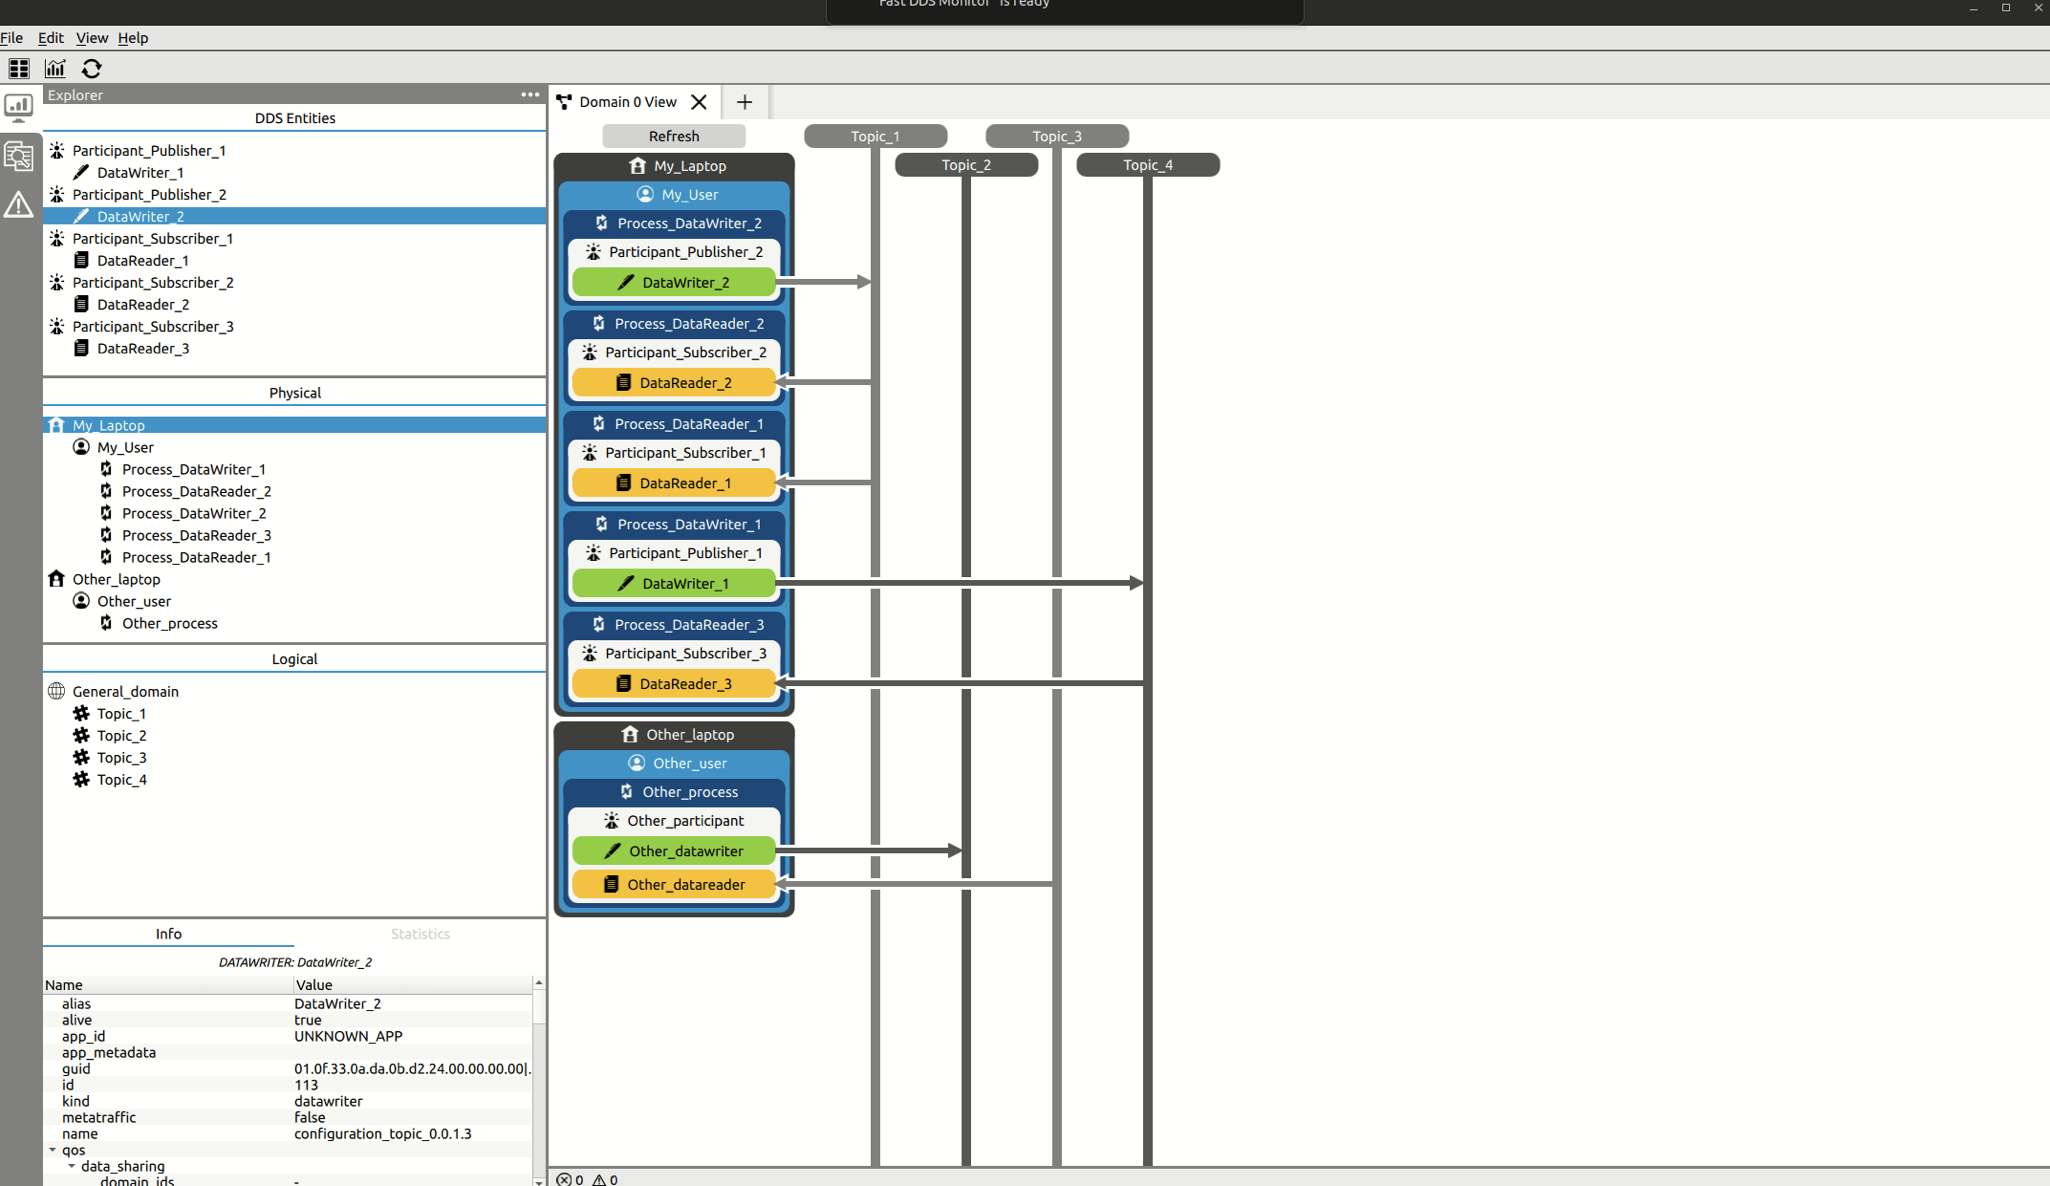
\includegraphics[width=1\textwidth]{Foto/DomainView.png}
		\caption{La figura che mostra il funzionamento del Domain View}
		\label{fig:DDS_DomainView}
	\end{figure}
	\item \textbf{Struttura logica DDS}: ogni processo è associato a uno o più \texttt{DomainParticipant}. Ogni partecipante espone i propri \texttt{DataWriter} (freccia in entrata nel topic, lato publisher) e \texttt{DataReader} (freccia in uscita dal topic, lato subscriber).
	
	\item \textbf{Visualizzazione del flusso dati}: nella Domain View, il topic è rappresentato come una linea verticale centrale. Il \texttt{Broadcastner} è visibile come il nodo con la freccia che punta \textit{verso} il topic (\texttt{DataWriter}), mentre il \texttt{Listener} è il nodo con la freccia che esce \textit{dal} topic (\texttt{DataReader}).
\end{itemize}

All'interno della Domain View sono disponibili funzionalità aggiuntive:
\begin{itemize}
	\item \textbf{Filtro per topic}: clic destro sul nome del topic $\rightarrow$ \textit{Filter topic graph}: apre una nuova scheda con il grafo filtrato per quel solo topic, utile quando la rete ha molti topic attivi contemporaneamente.
	\item \textbf{Visualizzazione IDL}: clic destro sul topic $\rightarrow$ \textit{Data type IDL view}: mostra la definizione IDL del tipo di messaggio, copiabile direttamente.
	\item \textbf{Cambio alias}: clic destro sull'entità $\rightarrow$ \textit{Change alias}: rinomina l'entità solo all'interno del monitor, senza modificare la rete DDS reale. Utile per distinguere rapidamente \texttt{Broadcastner} e \texttt{Listener} che FastDDS identifica entrambi come \texttt{RTPSParticipant}.
\end{itemize}

In questo progetto, la Domain View è stata utilizzata per verificare visivamente che il matching tra il \texttt{DataWriter} del \texttt{Broadcastner} e il \texttt{DataReader} del \texttt{Listener} fosse avvenuto correttamente prima di avviare il tracciamento con \texttt{trace-cmd}.

\clearpage

\subsection{Chart View: Visualizzazione Statistica della Comunicazione}

La \textbf{Chart View} è il cuore analitico del monitor. Permette di creare grafici personalizzati a partire dai topic statistici raccolti. Il monitor distingue due modalità di visualizzazione:
\begin{figure}[htbp]
	\centering
	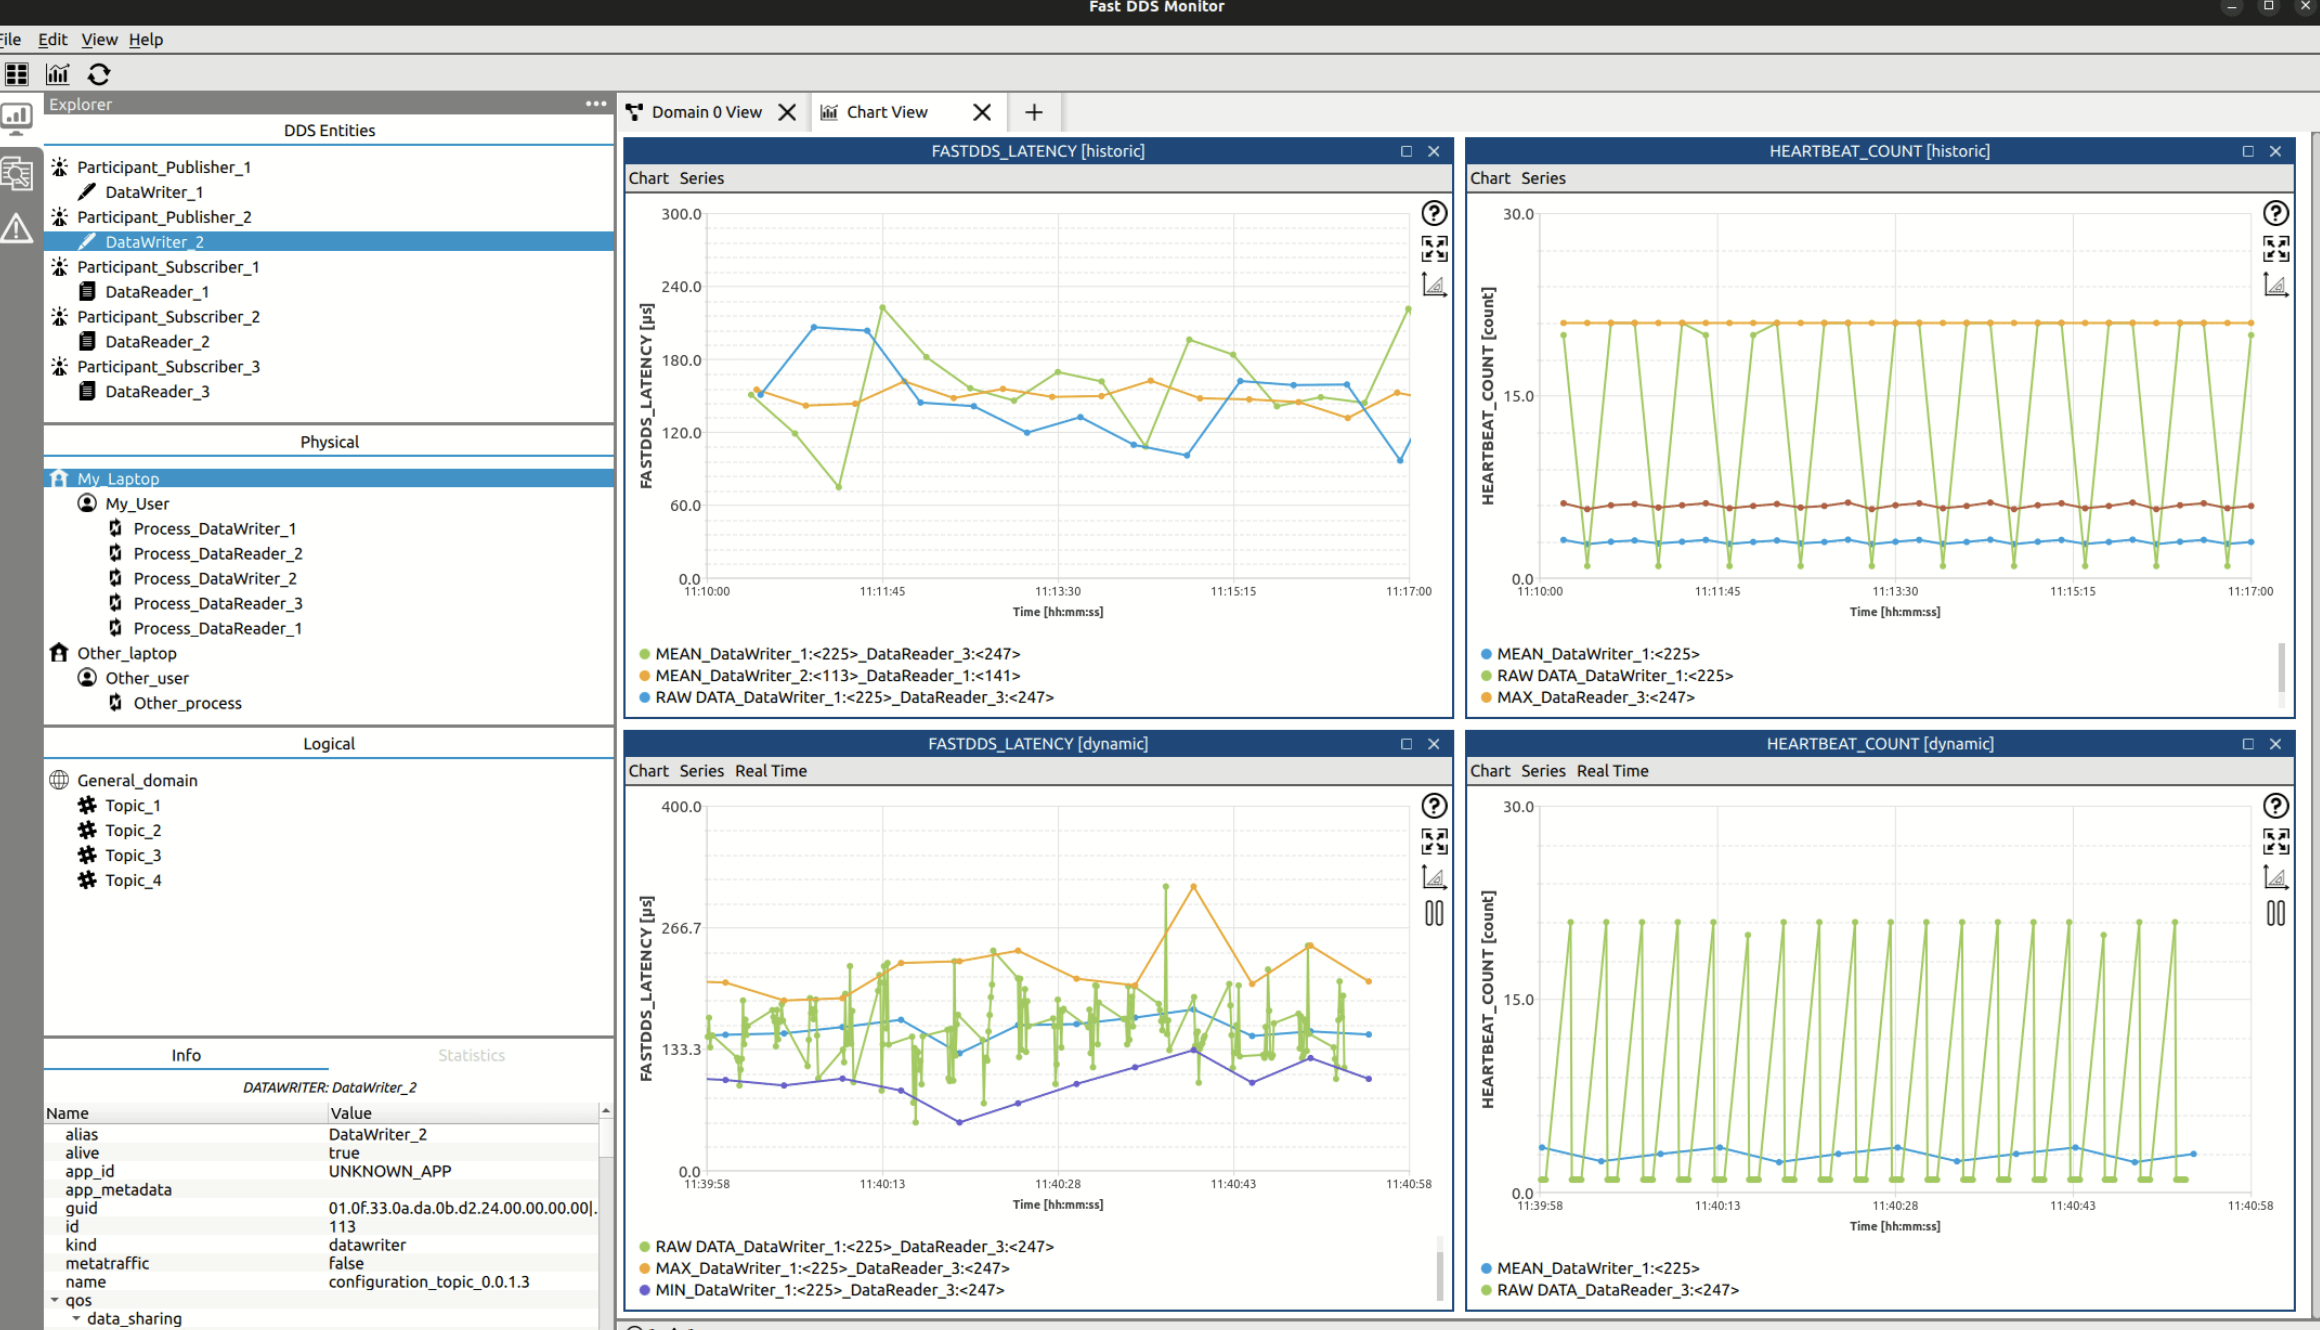
\includegraphics[width=0.90\textwidth]{Foto/Thread/DDS_Monitor}
	\caption{figura che mostra funzionamento del monitor DDS e del Chart View}
	\label{fig:DDS_Monitor}
\end{figure}

\subsubsection{Modalità di tracciamento statistico: }

La modalità storica interroga tutti i dati raccolti dal monitor dall'avvio fino al momento della creazione del grafico. I parametri configurabili sono:

\begin{itemize}
	\item \textbf{Topic statistico}: il tipo di metrica da visualizzare. I più rilevanti per questo progetto sono:
	\begin{itemize}
		\item \texttt{DATA\_COUNT}: numero di campioni pubblicati dal DataWriter in ogni intervallo temporale. Permette di verificare che il publisher stia inviando alla frequenza attesa (un campione ogni 600 ms per il task \texttt{DDS\_Publish}).
		\item \texttt{FASTDDS\_LATENCY}: tempo trascorso tra la chiamata \texttt{publish()} lato writer e la ricezione del dato nel callback \texttt{on\_data\_available()} lato reader. Questa è la metrica di latenza end-to-end più significativa per i sistemi RT.
		\item \texttt{PUBLICATION\_THROUGHPUT}: byte al secondo pubblicati dal writer, utile per verificare che lo streaming di immagini di \texttt{ImageSender} non saturi la banda disponibile.
		\item \texttt{NETWORK\_LATENCY}: latenza a livello di rete (RTPS transport), distinta dalla latenza applicativa. In un sistema su loopback o SHM, è tipicamente inferiore al microsecondo.
	\end{itemize}
	
	\item \textbf{Number of bins}: il numero di intervalli in cui suddividere la finestra temporale. Con \texttt{bins = 20}, i dati vengono aggregati in 20 punti. Con \texttt{bins = 0}, ogni singolo datapoint ricevuto viene visualizzato individualmente, mostrando la distribuzione grezza.
	
	\item \textbf{Statistics kind}: il tipo di aggregazione statistica applicata ai campioni in ogni bin:
	\begin{itemize}
		\item \texttt{MEAN}: media aritmetica (latenza media nell'intervallo).
		\item \texttt{MEDIAN}: mediana (meno sensibile agli outlier rispetto alla media).
		\item \texttt{MAX}: valore massimo (worst-case della latenza nel bin).
		\item \texttt{MIN}: valore minimo (best-case).
		\item \texttt{STANDARD\_DEVIATION}: deviazione standard (equivalente del Jitter per la latenza DDS).
		\item \texttt{SUM}: somma totale (utile con \texttt{DATA\_COUNT} per contare i messaggi totali inviati).
		\item \texttt{RAW\_DATA}: ogni singolo datapoint senza aggregazione.
	\end{itemize}
\end{itemize}

\paragraph{Esempio: grafico della latenza Broadcastner$\to$Listener.}
Per osservare la latenza di comunicazione nel progetto, si seleziona il topic \texttt{FASTDDS\_LATENCY}, si scelgono come entità sorgente il \texttt{DomainParticipant} del \texttt{Broadcastner} e come entità destinazione il \texttt{DomainParticipant} del \texttt{Listener}. Si aggiungono quattro serie con \texttt{Statistics kind} = \texttt{MEDIAN}, \texttt{MAX}, \texttt{MIN} e \texttt{STANDARD\_DEVIATION} per avere un quadro completo della distribuzione della latenza. 
\subsubsection{Dati in Tempo Reale}

La modalità real-time aggiorna il grafico automaticamente a intervalli configurabili, mostrando una finestra scorrevole dei dati più recenti:

\begin{itemize}
	\item \textbf{Time window}: la durata della finestra temporale visualizzata (es. 1 minuto). I dati più vecchi escono dalla finestra man mano che arrivano nuovi.
	\item \textbf{Update period}: ogni quanti secondi il monitor interroga il backend statistico per nuovi dati (es. ogni 5 secondi). Non rappresenta la frequenza di campionamento DDS, che avviene ad ogni messaggio ricevuto.
\end{itemize}

Nella modalità real-time, è possibile mettere in pausa l'aggiornamento degli assi per eseguire zoom e ispezione manuale dei dati (il pulsante play/pause), pur continuando a raccogliere nuovi campioni in background. Aggiungendo una serie con \texttt{RAW\_DATA} si visualizzano i singoli datapoint grezzi, permettendo di comprendere come \texttt{MEAN}, \texttt{MAX} e \texttt{MIN} vengano calcolati a partire da essi.

\subsubsection{Sistema di Allerta}

Il monitor offre un sistema di allerta configurabile: è possibile definire condizioni che, se soddisfatte, notificano l'utente o eseguono uno script automatico. I tipi di allerta sono:
\begin{itemize}
	\item \texttt{NEW\_DATA}: si attiva quando viene ricevuto un \texttt{DATA\_COUNT} positivo da un'entità corrispondente al filtro. Utile per rilevare che un publisher ha ripreso a inviare dopo un'interruzione.
	\item \texttt{NO\_DATA}: si attiva quando il \texttt{PUBLICATION\_THROUGHPUT} di un'entità scende sotto una soglia configurabile. Permette di rilevare automaticamente un publisher bloccato o lento.
\end{itemize}

In questo progetto, le allerte non sono state utilizzate attivamente, ma il sistema è stato usato per verificare visivamente che il \texttt{Broadcastner} non scendesse mai sotto la soglia di un messaggio per periodo (600 ms).
\clearpage
\subsection{Utilizzo nel Progetto: Validazione Prima del Tracciamento}

Il flusso di utilizzo del monitor DDS in questo progetto è il seguente:

\begin{enumerate}
	\item \textbf{Impostare la variabile d'ambiente} \texttt{FASTDDS\_STATISTICS} nel terminale prima dell'avvio dei nodi \texttt{Broadcastner} e \texttt{Listener}.
	\item \textbf{Avviare il monitor} e selezionare il domain ID corretto (lo stesso usato nel codice, es. \texttt{1}).
	\item \textbf{Verificare nella Domain View} che entrambi i processi siano visibili e che il matching DataWriter $\leftrightarrow$ DataReader sia stato stabilito correttamente.
	\item \textbf{Creare un grafico DATA\_COUNT} in modalità real-time per verificare che i messaggi vengano inviati alla frequenza attesa (circa 1.67 messaggi al secondo per il periodo di 600 ms).
	\item \textbf{Creare un grafico FASTDDS\_LATENCY} per misurare la latenza end-to-end prima di avviare il tracciamento kernel, in modo da avere un riferimento di confronto.
	\item Solo dopo aver validato la comunicazione DDS tramite il monitor, si avvia lo script \texttt{marker.sh} per il tracciamento congiunto dei due processi con \texttt{trace-cmd}.
\end{enumerate}

Questa procedura garantisce che eventuali problemi di configurazione DDS (es. domain ID sbagliato, QoS incompatibili, topic non trovato) vengano identificati e risolti \textbf{prima} di produrre un tracciato kernel che risulterebbe privo di eventi DDS significativi.

% =========================================================

\clearpage
\section{Strumenti di Tracciamento del Kernel: \texttt{ftrace}, \texttt{trace-cmd} e KernelShark}
\label{sec:tracecmd_kernelshark}


\subsection{Il Sottosistema \texttt{ftrace} del Kernel Linux}

\texttt{ftrace} è il framework di tracciamento integrato nel kernel Linux. Rappresenta lo strumento principale per il debug e il profiling del kernel senza necessità di modificare il codice sorgente del kernel o delle applicazioni \cite{rostedt_ftrace}. Espone un filesystem virtuale denominato \texttt{tracefs}, 
montato tipicamente in \texttt{/sys/kernel/debug/tracing/}  o \texttt{/sys/kernel/tracing/}, attraverso cui si interagisce direttamente con il sottosistema di tracciamento.

Il cuore di \texttt{ftrace} è il \textbf{buffer circolare per CPU}: il kernel mantiene un ring buffer separato per ogni core fisico. Quando un evento abilitato si verifica, il kernel scrive la relativa entry nel buffer del core su cui è in esecuzione con un timestamp ad alta risoluzione. La struttura per-CPU evita contese su lock globali, rendendo il meccanismo sufficientemente leggero da essere usato in sistemi Real-Time.

\subsubsection{I Tracepoint del Sottosistema \texttt{sched}}

Il sottosistema \texttt{sched} del kernel espone diversi tracepoint statici per la schedulazione. In questo progetto vengono utilizzati i seguenti \cite{tracecmd_record_man}:

\begin{itemize}
	\item \textbf{\texttt{sched:sched\_switch}}: registrato ad ogni cambio di contesto della CPU. Ogni evento cattura:
	\begin{itemize}
		\item \texttt{prev\_comm}, \texttt{prev\_pid}, \texttt{prev\_prio}: nome, PID e priorità del processo che abbandona la CPU.
		\item \texttt{prev\_state}: lo stato con cui il processo uscente si sospende:
		\begin{itemize}
			\item \texttt{S} (\textit{Sleeping}): sospensione volontaria (es. \texttt{clock\_nanosleep}).
			\item \texttt{R} (\textit{Runnable}): il processo è pronto ma è stato prelazionato da uno a priorità maggiore.
			\item \texttt{D} (\textit{Uninterruptible sleep}): bloccato su I/O o mutex kernel.
		\end{itemize}
		\item \texttt{next\_comm}, \texttt{next\_pid}, \texttt{next\_prio}: nome, PID e priorità del processo subentrante.
	\end{itemize}
	Questo evento è il dato primario da cui il parser C++ ricostruisce gli intervalli \texttt{RUN}, \texttt{SLEEP} e \texttt{PREEMPT} di ogni task 
	
	\item \textbf{\texttt{sched:sched\_wakeup}}: registrato quando un thread viene estratto dallo stato di sleep e inserito nella coda di pronto. La differenza temporale tra questo evento e il successivo \texttt{sched\_switch} che porta il thread in esecuzione è la \textbf{latenza di attivazione} (\textit{wakeup latency}), una metrica critica nei sistemi RT.
	
	\item \textbf{\texttt{tracing\_mark\_write}}: questo non è un tracepoint kernel ma un meccanismo di iniezione dallo spazio utente. Qualsiasi stringa scritta dall'applicazione nel file virtuale \texttt{/sys/kernel/debug/tracing/trace\_marker} (tramite la funzione \texttt{write\_trace\_marker()} del progetto) viene inserita nel ring buffer del core corrente con il timestamp al nanosecondo del kernel, sincronizzato con gli eventi \texttt{sched\_switch}. Questa sincronizzazione è il fondamento dell'intera pipeline di analisi: permette di correlare i marker applicativi (es. \texttt{PERIOD\_START\_Activity\_1}) con i cambi di contesto reali del kernel.
\end{itemize}

\subsection{\texttt{trace-cmd}: Interfaccia a Riga di Comando per \texttt{ftrace}}

\texttt{trace-cmd} è il tool in spazio utente  che semplifica l'uso di \texttt{ftrace} \cite{tracecmd_record_man}. Internamente, \texttt{trace-cmd record} crea un processo di registrazione separato per ogni CPU disponibile: questi processi leggono continuamente il ring buffer del proprio core e scrivono i dati in file temporanei. Al termine della sessione, tutti i file temporanei vengono concatenati nel file binario compresso \texttt{trace.dat}.

\subsubsection{Utilizzo in \texttt{run\_trace.sh}: Tracciamento di un Singolo Processo}

Negli script \texttt{run\_trace.sh} e \texttt{run\_trace\_dds.sh}, \texttt{trace-cmd record} viene invocato nella sua modalità più diretta: avvia l'eseguibile e registra simultaneamente gli eventi del kernel per tutta la sua durata:

\begin{lstlisting}[language=bash, caption={Invocazione di trace-cmd record in run\_trace.sh}]
	sudo trace-cmd record \
	-e sched:sched_switch \   # abilita il tracepoint sched_switch
	-e sched:sched_wakeup \   # abilita il tracepoint sched_wakeup
	-o "$OUTPUT_DIR/trace.dat" \  # file di output binario nella sandbox
	"$EXECUTABLE"             # avvia l'eseguibile e lo traccia
\end{lstlisting}

I parametri hanno il seguente significato preciso:

\begin{itemize}
	\item \textbf{\texttt{-e sched:sched\_switch}}: abilita il tracepoint \texttt{sched\_switch} nel sottosistema \texttt{sched}. Secondo la documentazione ufficiale \cite{tracecmd_record_man}, il formato dell'argomento è \texttt{subsystem:event-name}; è anche possibile abilitare tutti gli eventi di un sottosistema omettendo il nome dell'evento (es. \texttt{-e sched}).
	
	\item \textbf{\texttt{-e sched:sched\_wakeup}}: abilita il tracepoint \texttt{sched\_wakeup}. L'aggiunta di questo evento, pur aumentando leggermente il volume del log, è fondamentale per misurare la latenza tra il risveglio di un thread (fine del \texttt{clock\_nanosleep}) e il momento in cui ottiene effettivamente la CPU (\texttt{sched\_switch} con \texttt{next\_pid} corrispondente).
	
	\item \textbf{\texttt{-o \$OUTPUT\_DIR/trace.dat}}: specifica il percorso del file di output. Ogni sessione viene salvata in una sandbox con timestamp univoco (es. \texttt{bin/Test/trace\_results
		\_app10g\_20260427\_212626/}), garantendo che nessuna sessione sovrascriva un'altra.
	
	\item \textbf{Argomento posizionale \texttt{\$EXECUTABLE}}: quando un comando viene passato a \texttt{trace-cmd record} come ultimo argomento, il tool lo avvia e interrompe automaticamente la registrazione al termine del processo. Se nessun comando viene specificato, la registrazione continua finché l'utente non preme \texttt{Ctrl-C}: questa è la modalità usata negli script \texttt{marker.sh}.
\end{itemize}

In questo caso \textbf{non} viene usata l'opzione \texttt{-P} (filtraggio per PID) perché l'eseguibile viene avviato direttamente da \texttt{trace-cmd}: il tool conosce già il PID del processo figlio e filtra automaticamente. Tutti gli eventi degli altri processi del sistema vengono scartati dal kernel prima ancora di essere scritti nel ring buffer, riducendo il volume del log.

\subsubsection{Utilizzo in \texttt{marker.sh}: Tracciamento Passivo Multi-Processo}

Negli script \texttt{marker.sh} e \texttt{marker1.sh}, la modalità di utilizzo è sostanzialmente diversa: i processi sono già in esecuzione quando lo script viene avviato, quindi non si può usare il meccanismo di lancio diretto. Si usa invece l'opzione \texttt{-P} per specificare esplicitamente i PID da tracciare:

\begin{lstlisting}[language=bash, caption={Invocazione di trace-cmd record in marker.sh con filtraggio per PID}]
	# PIDS_CMD viene costruita iterativamente durante la fase di aggancio:
	# PIDS_CMD="-P 9120 -P 9121 -P 9122 -P 9200 -P 9201"
	# (PID del processo principale + TID di ogni thread interno)
	
	sudo trace-cmd record \
	-e sched:sched_switch \
	-e sched:sched_wakeup \
	$PIDS_CMD \               # filtra SOLO i thread elencati
	-o "$OUTPUT_DIR/trace.dat"
	# Nessun eseguibile: registra finche' l'utente preme Ctrl-C
\end{lstlisting}

La differenza critica rispetto a \texttt{run\_trace.sh} è l'assenza dell'eseguibile finale: senza un comando da lanciare, \texttt{trace-cmd} registra fino all'interruzione manuale (\texttt{Ctrl-C}). Questo permette di controllare esattamente la durata della sessione di tracciamento, indipendentemente dalla vita dei processi.

L'opzione \texttt{-P} (per PID, equivalente a \texttt{-F} che filtra solo il processo figlio, ma per PID già esistenti) istruisce il kernel a registrare eventi di scheduling solo quando il thread \texttt{prev\_pid} o \texttt{next\_pid} dell'evento \texttt{sched\_switch} corrisponde a uno dei PID specificati. Questo filtraggio avviene \textbf{nel kernel}, non nel tool in user space: significa che i thread non elencati non generano mai entries nel ring buffer, eliminando completamente il rumore di sistema.

\subsubsection{Il File Prodotto: \texttt{trace.dat}}

Il file \texttt{trace.dat} è un archivio binario proprietario del formato \texttt{trace-cmd}. Non è leggibile direttamente da un editor di testo: contiene i metadati del sistema (versione del kernel, numero di CPU, mappa degli eventi abilitati con i loro formati), seguiti dai dati grezzi di ogni CPU compressi \cite{tracecmd_record_man}. La dimensione tipica per una sessione di 5-10 secondi con i soli eventi \texttt{sched\_switch} e \texttt{sched\_wakeup} è dell'ordine di pochi MB.

\subsection{Il Comando \texttt{trace-cmd report}: Decodifica del Log Binario}

Al termine della registrazione, il file binario \texttt{trace.dat} viene decodificato in un report testuale tramite \texttt{trace-cmd report}. Negli script del progetto, la decodifica avviene sempre con la stessa sintassi:

\begin{lstlisting}[language=bash, caption={Decodifica del log binario negli script run\_trace.sh e marker2.sh}]
	# Necessario perche' trace-cmd record ha girato con sudo
	sudo chown -R "$(id -u):$(id -g)" "$OUTPUT_DIR"
	
	# Decodifica: legge trace.dat e produce il report testuale
	trace-cmd report "$OUTPUT_DIR/trace.dat" > "$OUTPUT_DIR/trace_output.txt"
\end{lstlisting}

Il comando \texttt{trace-cmd report} legge il file \texttt{trace.dat}, interpreta i metadati per conoscere il formato di ogni evento (numero e tipo dei campi), e serializza ogni entry del ring buffer in una riga testuale nel formato standard \cite{tracecmd_record_man}:

\begin{lstlisting}[caption={Formato delle righe in trace\_output.txt }]
	comm-PID [CPU] timestamp: evento: dettagli
	
	# Esempi reali:
	Activity_1-8272  [001]  1234.567810: print:          tracing_mark_write: PERIOD_START_Activity_1
	Activity_1-8272  [001]  1234.567890: sched_switch:   prev_comm=Activity_1 prev_pid=8272
	prev_prio=98 prev_state=S
	==> next_comm=swapper/1 next_pid=0 next_prio=120
	swapper/1-0      [001]  1234.768000: sched_wakeup:   comm=Activity_1 pid=8272 prio=98
	target_cpu=001
	Activity_1-8272  [001]  1234.768050: sched_switch:   prev_comm=swapper/1 prev_pid=0
	==> next_comm=Activity_1 next_pid=8272
	Activity_1-8272  [001]  1234.768060: print:          tracing_mark_write: PERIOD_END_Activity_1
\end{lstlisting}

L'analisi di questa sequenza illustra la correlazione fondamentale che il parser C++ usa.

\begin{enumerate}
	\item Il marker \texttt{PERIOD\_START\_Activity\_1} a $t = 1234.567810$ segnala l'inizio del ciclo.
	\item Il \texttt{sched\_switch} con \texttt{prev\_state=S} a $t = 1234.567890$ mostra che il task si è sospeso volontariamente (ha chiamato \texttt{clock\_nanosleep}): inizia un intervallo \texttt{SLEEP}.
	\item Il \texttt{sched\_wakeup} a $t = 1234.768000$ mostra che il timer ha risvegliato il task: finisce il \texttt{SLEEP}.
	\item Il \texttt{sched\_switch} a $t = 1234.768050$ con \texttt{next\_pid=8272} mostra che il task ha ottenuto la CPU: il gap tra questo evento e il precedente risveglio ($50\ \mu$s) è la latenza di attivazione.
	\item Il marker \texttt{PERIOD\_END\_Activity\_1} a $t = 1234.768060$ conclude il ciclo.
\end{enumerate}

\noindent\textbf{File prodotto:} \texttt{bin/Test/trace\_results\_<app>\_<timestamp>/trace\_output.txt}


\clearpage
\subsection{KernelShark: Visualizzazione Grafica del Tracciato}

\textbf{KernelShark} è la GUI ufficiale per la visualizzazione dei file \texttt{trace.dat}, sviluppata da Steven Rostedt. \cite{rostedt_ftrace}. Il suo utilizzo è integrato negli script \texttt{marker.sh} del progetto:
\begin{figure}[htbp]
	\centering
	
\includegraphics[width=0.40\textwidth]{Foto/Thread/KernelShark.png}
	\caption{logo dell applicazione}
	\label{fig:KernelShark}
\end{figure}
\begin{lstlisting}[language=bash, caption={Apertura automatica di KernelShark negli script marker}]
	if command -v kernelshark >/dev/null 2>&1; then
	(cd "$OUTPUT_DIR" && kernelshark trace.dat) &
	fi
\end{lstlisting}

L'apertura avviene in un sottoprocesso in background (\texttt{\&}) per non bloccare il completamento dello script. KernelShark viene lanciato nella directory della sandbox corrente in modo che possa trovare il file \texttt{trace.dat} con un percorso relativo.

Le funzionalità usate in questo progetto sono:

\begin{itemize}
	\item \textbf{Timeline per core}: ogni riga della vista principale corrisponde a un core fisico e mostra i processi attivi in ogni istante con barre colorate. È possibile identificare visivamente i periodi di \texttt{SLEEP} (barre brevi) e i momenti di prelazione (cambio di colore senza transizione allo \texttt{swapper}).
	
	\item \textbf{Filtro per thread}: cliccando su un thread nel pannello laterale, si visualizzano solo gli eventi di quel thread sull'intera timeline, permettendo di isolare il comportamento di un singolo task (es. solo \texttt{Activity\_1}) in un tracciato con 20 thread.
	
	\item \textbf{Visualizzazione dei marker}: gli eventi \texttt{tracing\_mark\_write} (marker scritti dall'applicazione) appaiono come etichette testuali sulla timeline, sovrapposte ai corrispondenti eventi di scheduling. Questo permette di validare visivamente che i marker \texttt{PERIOD\_START}/\texttt{FUNCTION\_START}/\texttt{FUNCTION\_END}/\texttt{PERIOD\_END} cadano negli istanti attesi.
	
	\item \textbf{Zoom e cursori}: due cursori verticali permettono di selezionare un intervallo temporale e misurarne la durata con precisione al microsecondo, utile per verificare manualmente i valori di WCET e Jitter calcolati dal parser C++.
	\begin{figure}[htbp]
		\centering
		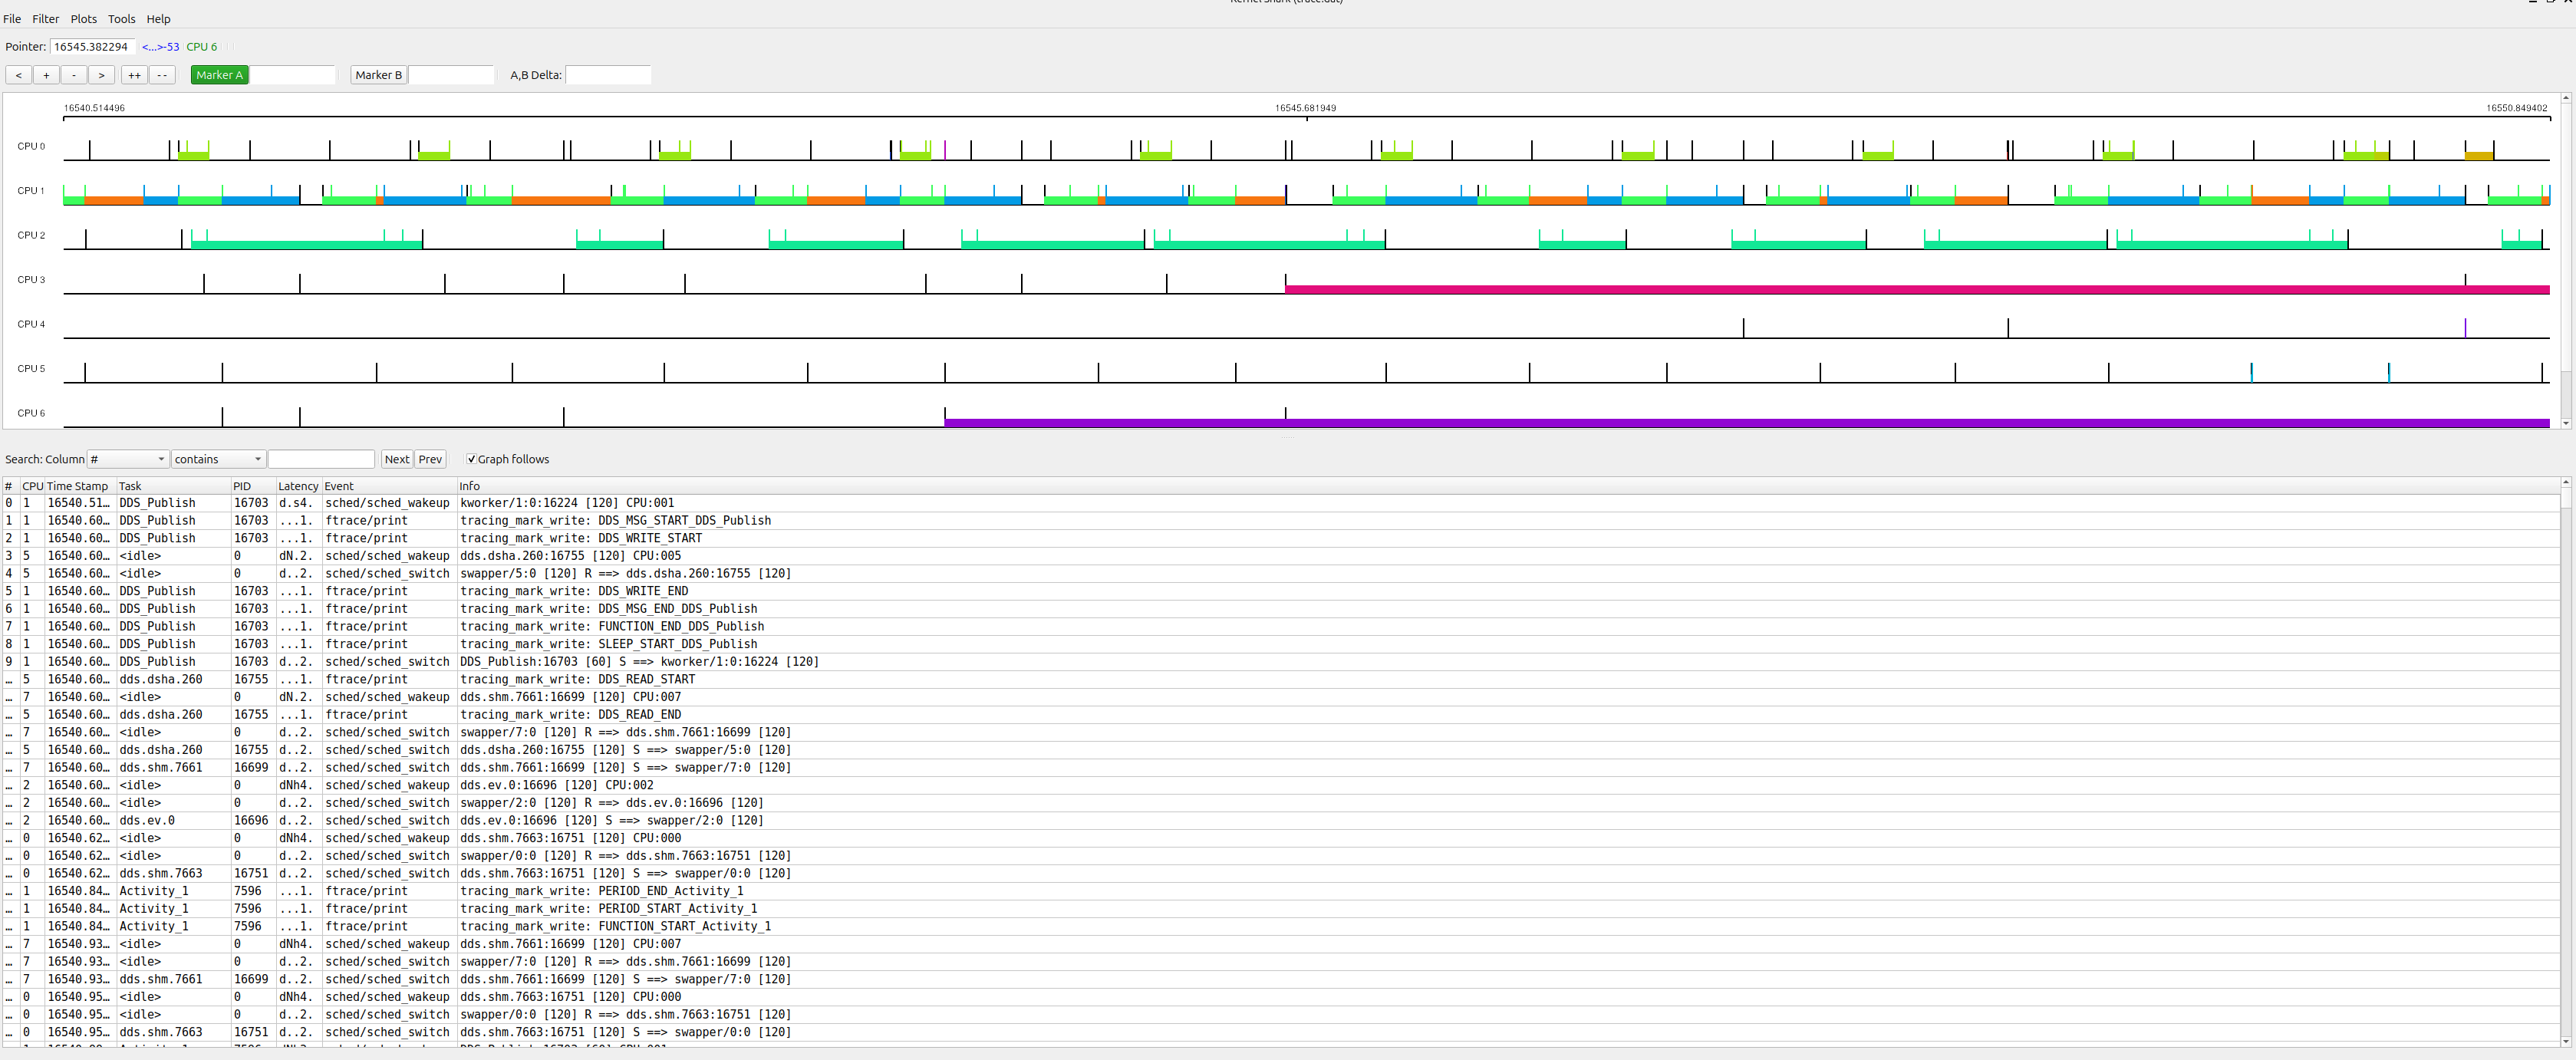
\includegraphics[width=1\textwidth]{Foto/Thread/SharkBroadcastner.png}
		\caption{Interfacccia grafica di KernelShark}
		\label{fig:interfaccia_KernelShark}
	\end{figure}
\end{itemize}




% ============================================================
\subsection{La Dashboard: \texttt{dashboard.py}}
\label{sec:dashboard}
% ============================================================

\noindent\textbf{Posizione nel progetto:} \texttt{src/tools/dashboard.py}

\bigskip


Tutte le operazioni descritte nei capitoli precedenti (avvio delle applicazioni, scelta dello script di tracciamento, controllo della registrazione, analisi e visualizzazione) richiedono tradizionalmente l'apertura di più terminali in parallelo, ricordando l'ordine corretto degli script e gestendo manualmente i percorsi. La \texttt{dashboard.py} nasce per eliminare questa complessità operativa: è un'interfaccia grafica desktop realizzata in Python che unifica in un'unica finestra l'intero flusso di lavoro del progetto.

L'applicazione si avvia senza necessità di argomenti, calcola automaticamente la radice del progetto e gestisce nativamente l'escalation dei privilegi (\texttt{sudo}) richiedendo la password una sola volta per l'intera sessione, senza memorizzarla su disco in modo permanente. La finestra è organizzata in tre \textit{tab} (schede) principali, selezionabili dalla barra superiore: \textit{Scripts Manager (Single)}, \textit{DDS Studio (Multi)} e \textit{Trace Manager}.


\subsection{Prerequisiti di Installazione}
Appena scaricato il progetto, prima di avviare gli strumenti di tracciamento o la dashboard, è strettamente necessario soddisfare le dipendenze di sistema. All'interno della cartella \texttt{bin/tools/} sono forniti due script eseguibili automatizzati per questo scopo:
\begin{itemize}
	\item \texttt{install\_project\_deps.sh}: provvede ad installare le librerie Python (come \texttt{pandas}, \texttt{matplotlib}, \texttt{tkinter}, \texttt{Pillow}) e i pacchetti di sistema essenziali per la compilazione.
	\item \texttt{install\_kernelshark.sh}: automatizza l'installazione di \texttt{trace-cmd} e dell'interfaccia grafica \texttt{kernelshark}, indispensabili per l'acquisizione e la visualizzazione del tracciato kernel.
	\item \texttt{script per lancio della dashboard}: per avviare la dashboard si può lanciare lo script presente in \texttt{bin/tools}, in questo modo ./run\_dashboard.sh
\end{itemize}
Questi script sollevano l'utente dalla noiosa configurazione manuale dell'ambiente.

\clearpage
% ============================================================
\subsubsection{Tab 1: Scripts Manager}
% ============================================================
Questa scheda della dashboard è dedicata all'avvio e al tracciamento di applicazioni a singolo processo (come \texttt{app10g}). Il flusso è diviso in due passaggi. A sinistra è presente la lista degli script Bash (\texttt{marker1.sh}, \texttt{run\_trace.sh}, ecc.). A destra l'utente seleziona il \textit{Target Process to Trace} da un menu a tendina che scansiona automaticamente la cartella \texttt{bin/app}. I bottoni di avvio permettono di lanciare lo script in background (con l'output reindirizzato alla console integrata) oppure in un emulatore di terminale esterno. Il bottone di arresto invia un segnale \texttt{SIGINT} simulando il \texttt{Ctrl+C}. Se lo script eseguito è di tipo \texttt{marker}, al termine viene proposto automaticamente di completare la pipeline di analisi (parsing e generazione grafici).

\begin{figure}[htbp]
	\label{tab:Scripts_Manager}
	\centering
	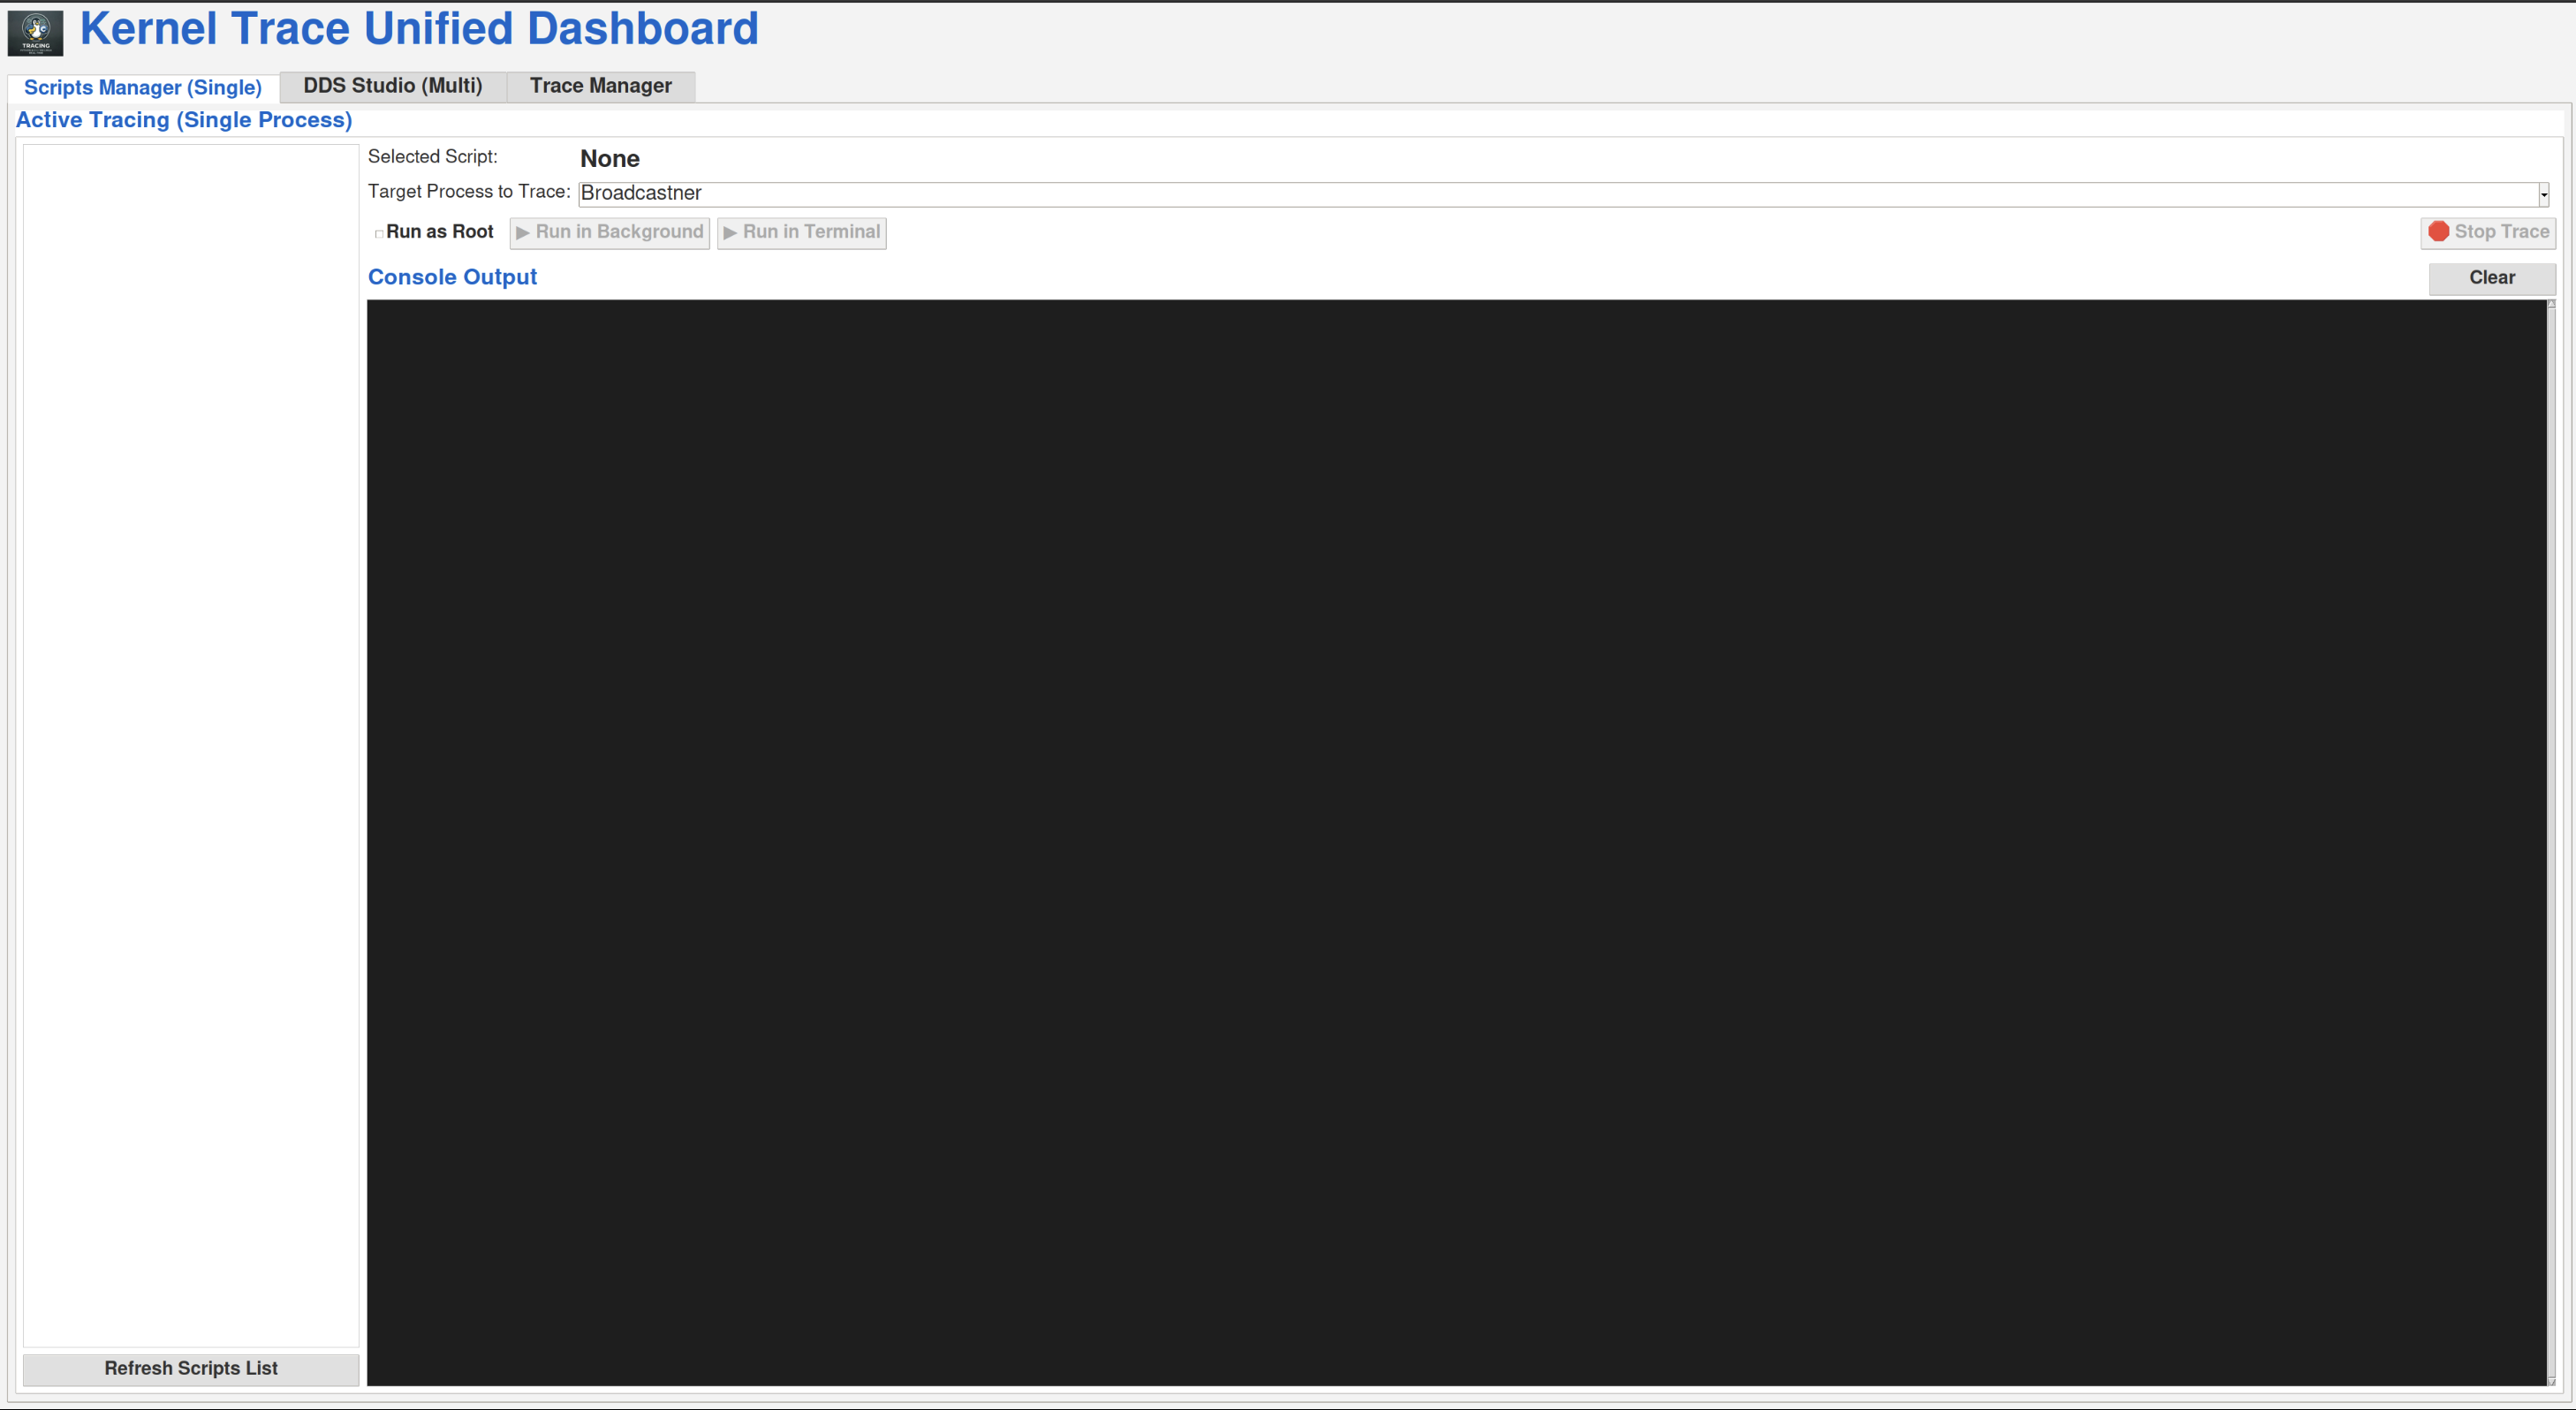
\includegraphics[width=0.8\textwidth]{Foto/Thread/ScriptsManager.png}
	\caption{Tab presente nella dashboard per il tracing di singoli processi}

\end{figure}
% ============================================================
\subsubsection{Tab 2: DDS Studio MultiProcesso}
% ============================================================
Questa scheda estende le funzionalità della precedente per gestire le applicazioni di comunicazione distribuita (come \texttt{Broadcastner} e \texttt{Listener}). L'utente può popolare una lista multipla di processi target e, con un singolo click su \textit{Launch ALL}, avviare automaticamente tutti i terminali necessari con i rispettivi eseguibili. Allo stesso modo, avviando uno script di tracciamento (es. \texttt{marker\_dds.sh}), la GUI preleva automaticamente tutti i processi dalla lista e li passa in sequenza allo script Bash, istruendo \texttt{trace-cmd} a tracciare l'intero sistema distribuito in modo trasparente.
\begin{figure}[H]
	\label{tab:DDS_Studio}
	\centering
	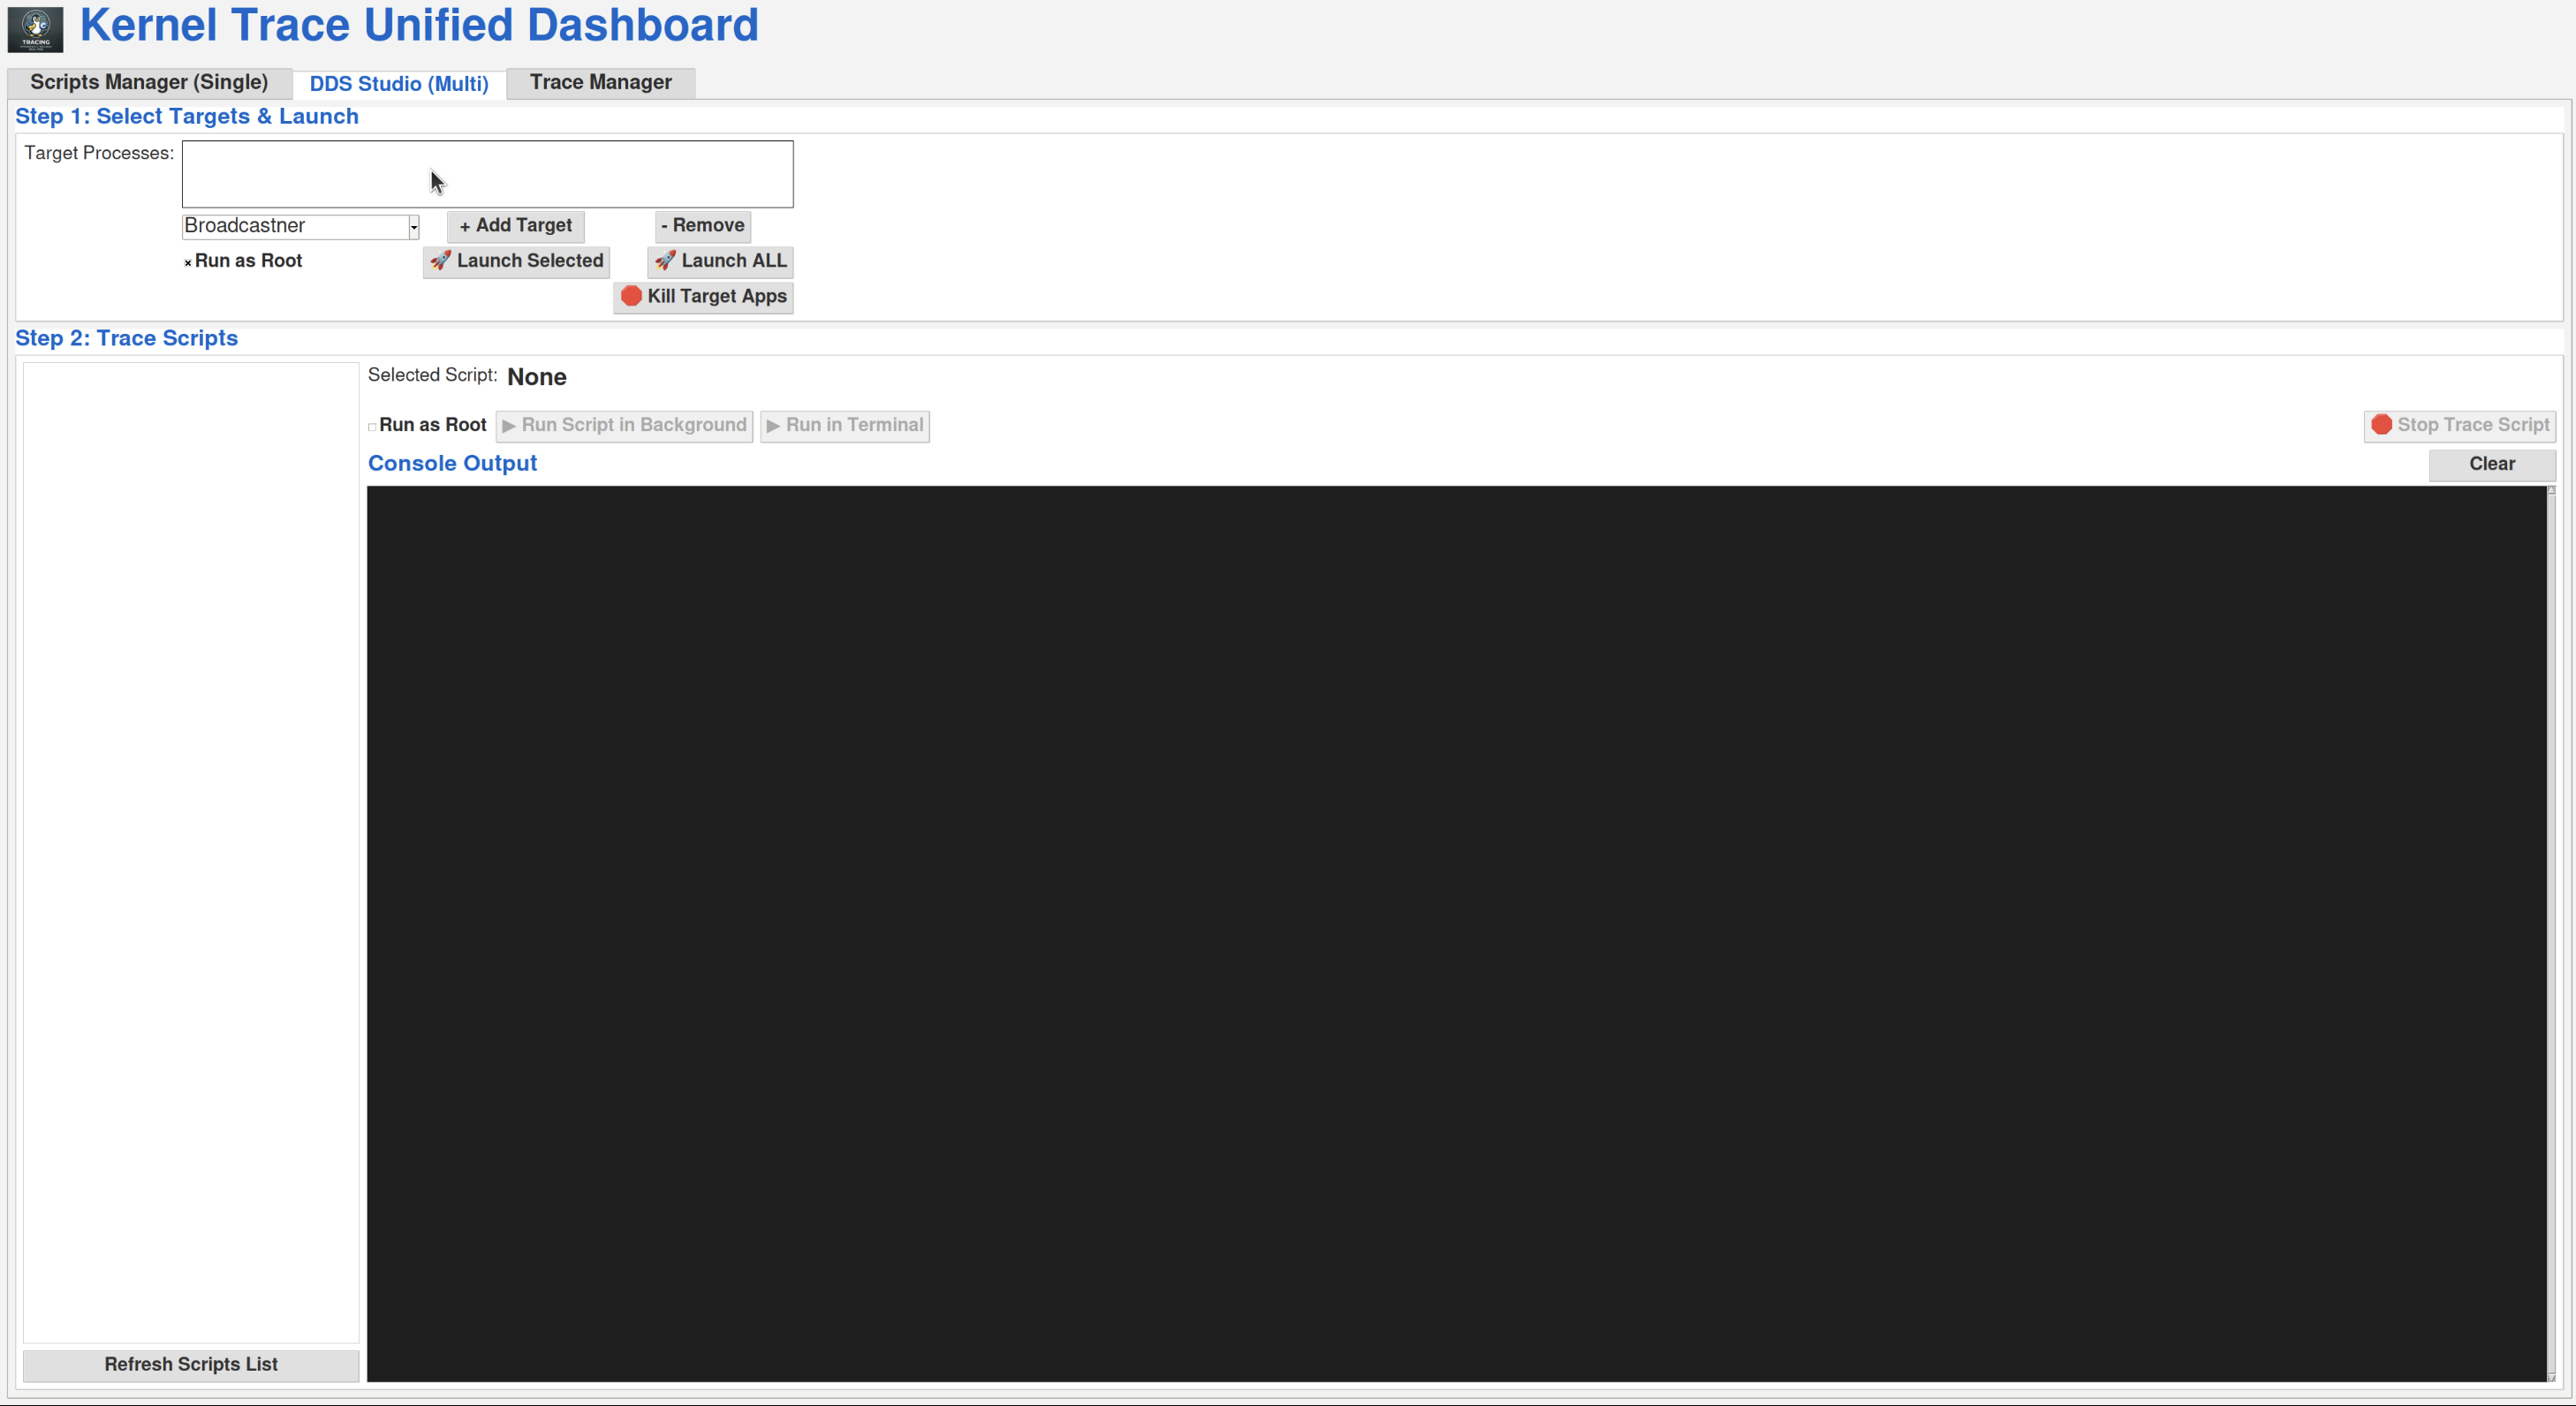
\includegraphics[width=0.8\textwidth]{Foto/Thread/DDS_Studio.png}
	\caption{tab per il tracing di più processi nella dashboard}

\end{figure}
% ============================================================
\subsubsection{Tab 3: Trace Manager}
% ============================================================
Questa scheda funge da archivio e visualizzatore rapido delle sessioni prodotte archiviate in \texttt{bin/Test/}. Il \textit{Trace Manager} mostra tutte le sessioni ordinate cronologicamente. Selezionando una voce, il pannello destro mostra l'elenco dei file con le rispettive dimensioni e il resoconto testuale (\texttt{risultati\_finali.txt}). 

I bottoni superiori permettono di interagire con la sessione:
\begin{itemize}
    \item \textbf{Open KernelShark}: avvia l'interfaccia di visualizzazione leggendo il \texttt{trace.dat}.
    \item \textbf{View Monitor Image}: apre l'immagine PNG prodotta dal monitor Python.
    \item \textbf{Delete Trace}: elimina la cartella della sessione di test.
\end{itemize}
\begin{figure}[H]
	\label{tab:TraceManager}
	\centering
	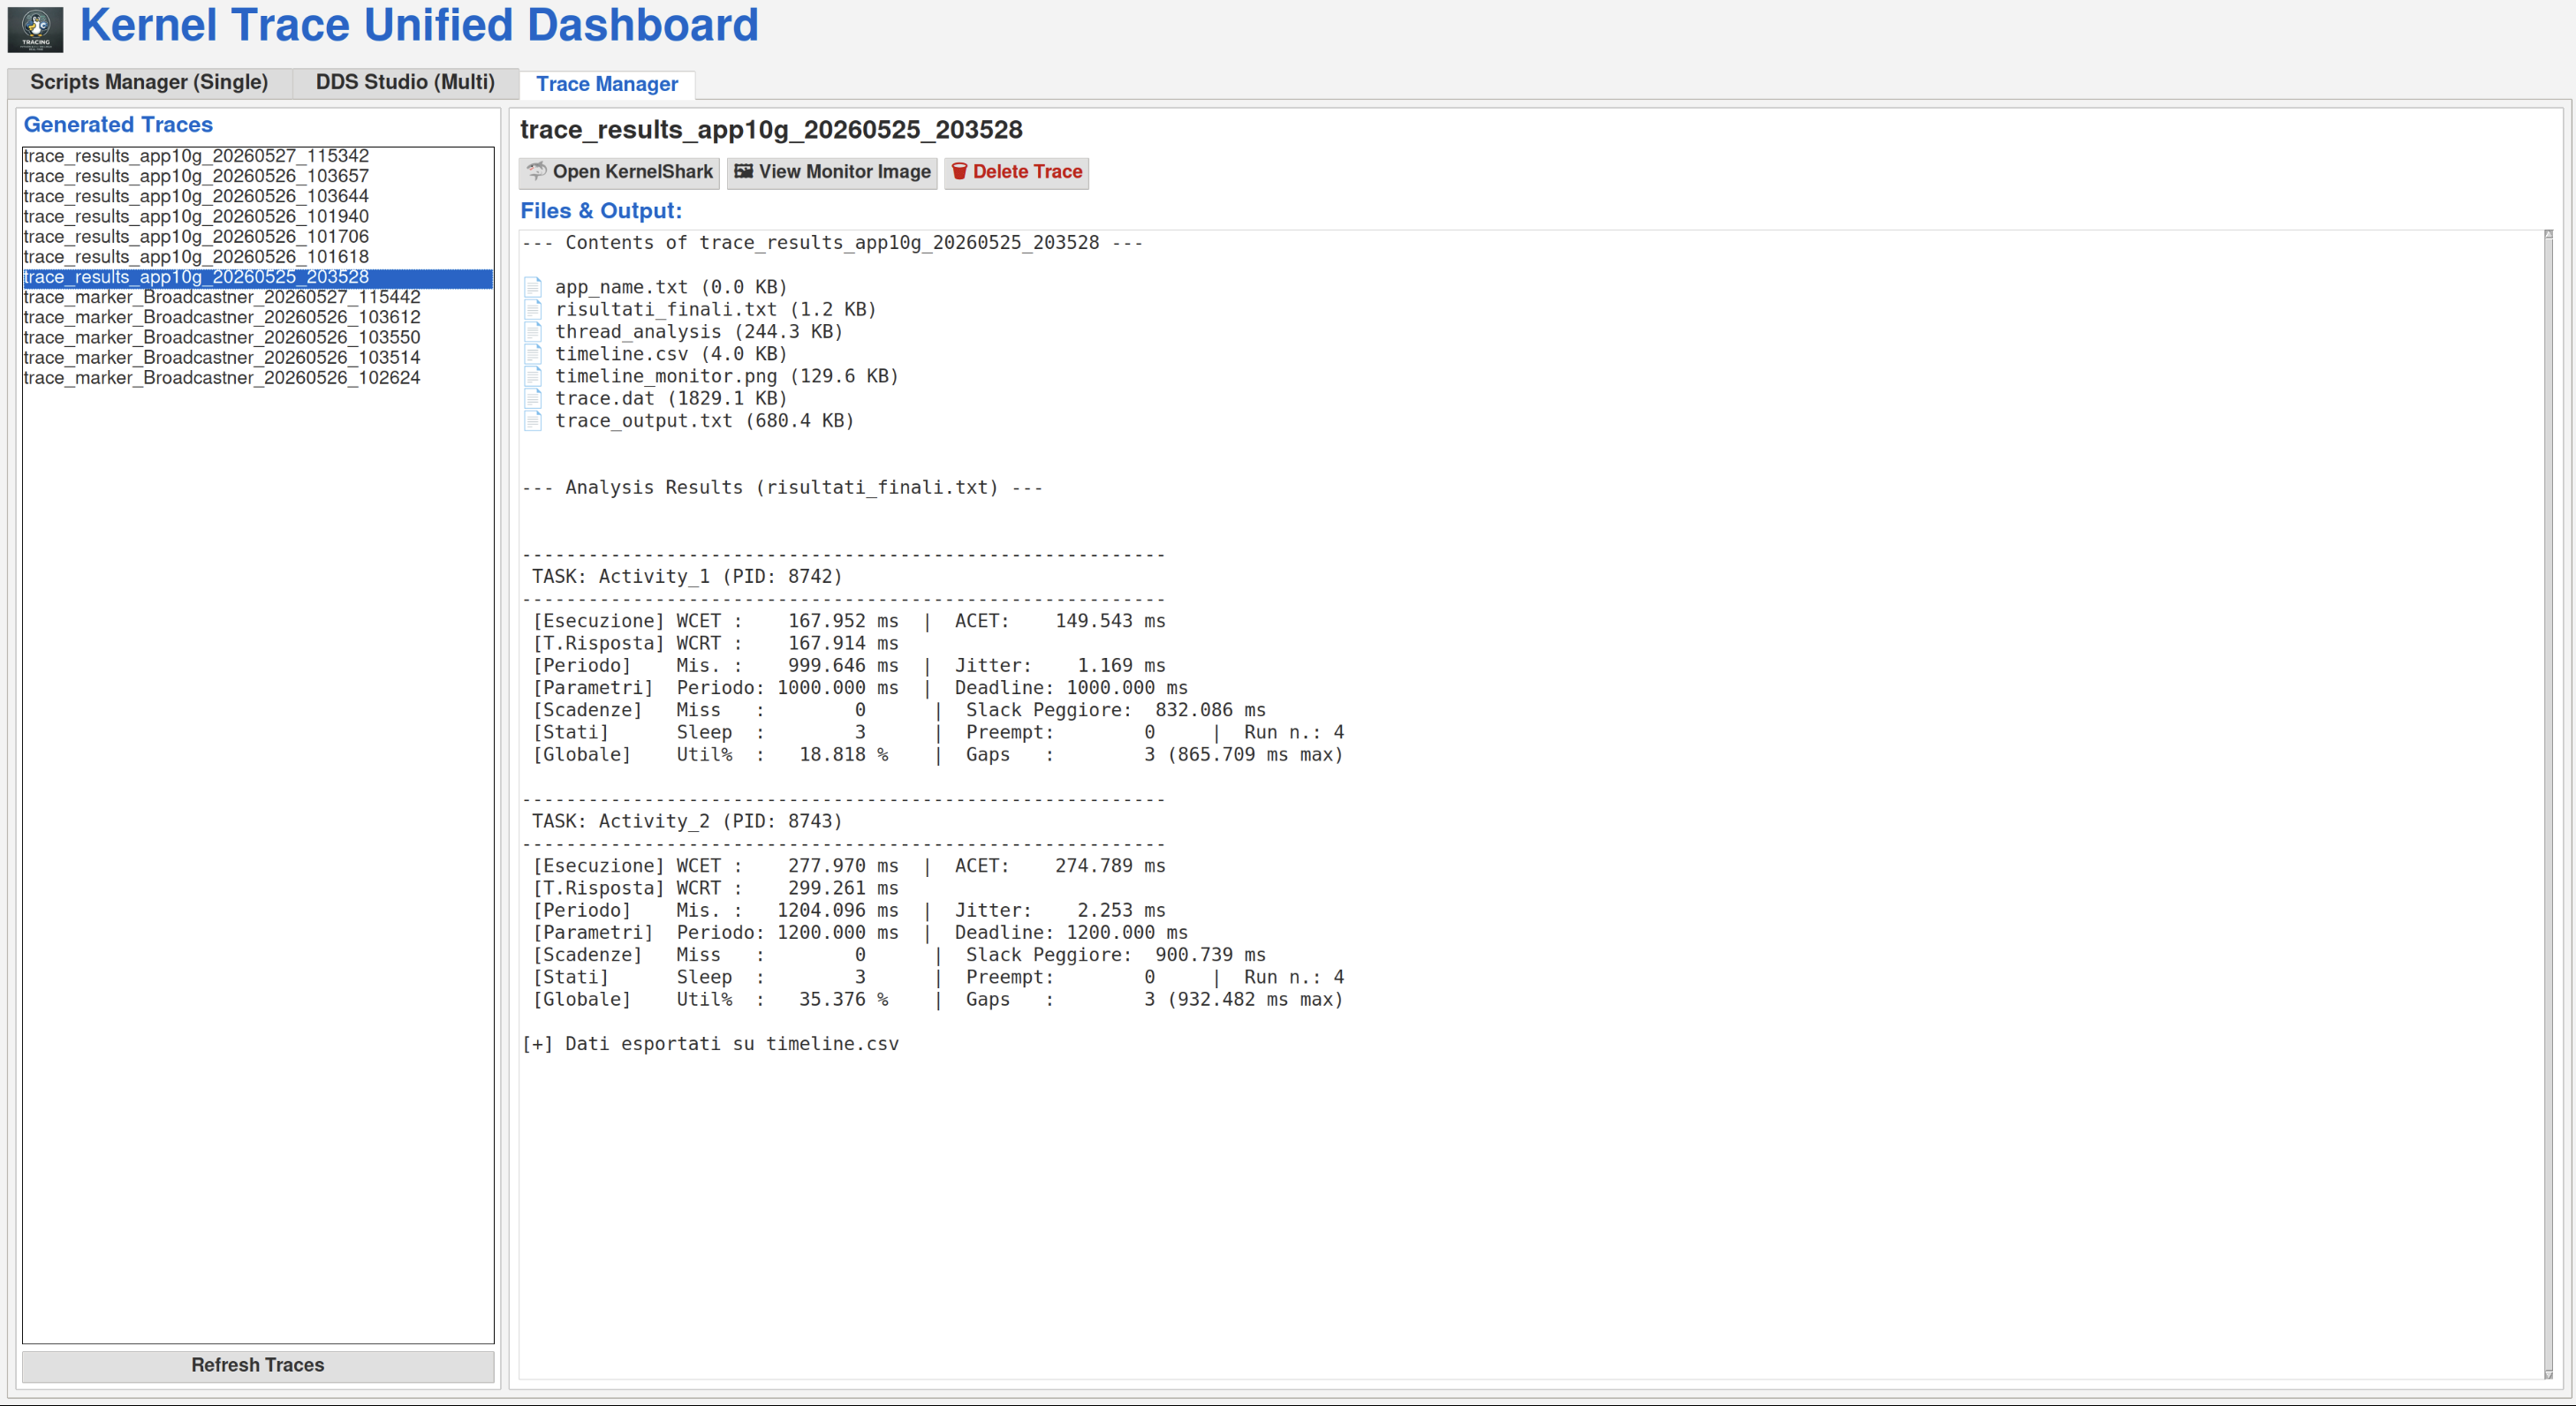
\includegraphics[width=0.8\textwidth]{Foto/Thread/Trace_Manager.png}
	\caption{}
	
\end{figure}

\clearpage
\subsection{Flow-Chart di Riferimento per ottenere i Documenti di Progetto}

Il flusso completo dall'acquisizione alla visualizzazione è riassunto nel flow-chart seguente, che descrive i file prodotti a ogni step.

\begin{figure}[htbp]
	\label{tab:pipeline_files}
	\centering
	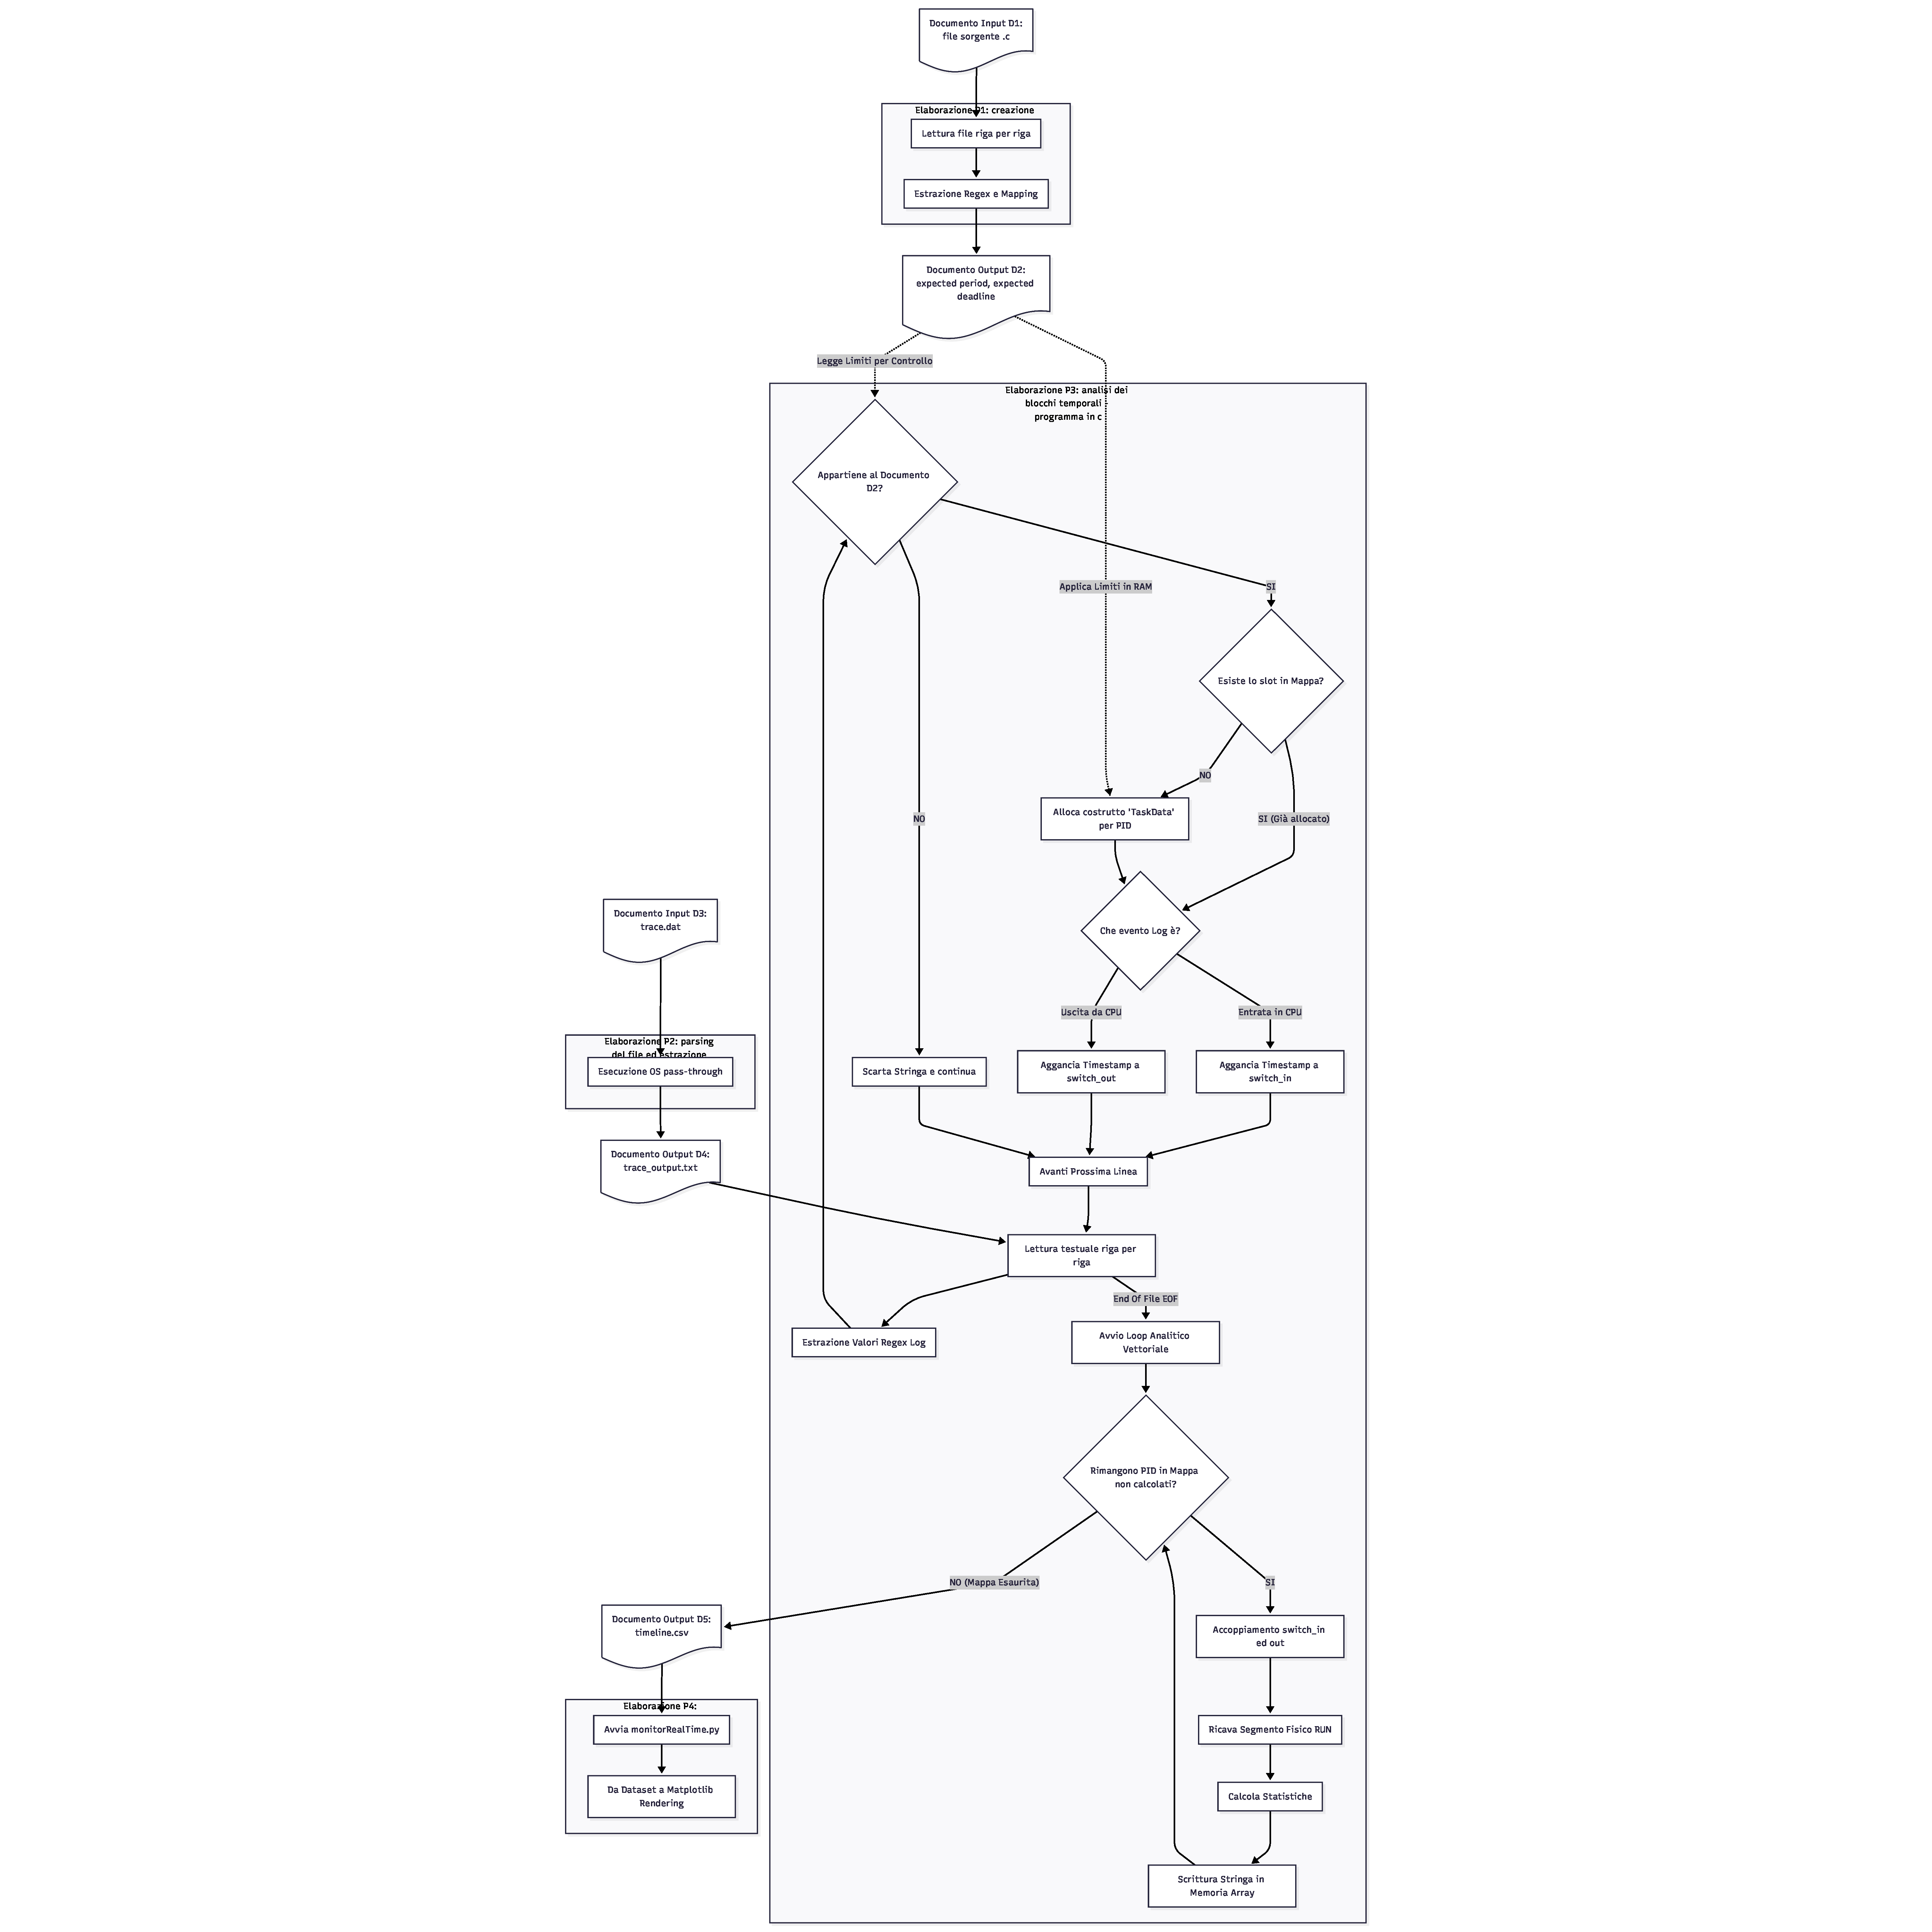
\includegraphics[width=0.9\textwidth]{Foto/Thread/flowchart.pdf}
	\caption{Flowchart di riferimento e flusso dati}
	\label{fig:flowchart}
\end{figure}
\clearpage

\section{Librerie Python Utilizzate}
\label{sec:python_libs}

I tool sviluppati in questo progetto, come il monitor grafico (\texttt{monitor.py}) e l'interfaccia unificata (\texttt{dashboard.py}), si affidano a diverse librerie  Python:

\subsection{Librerie per l'Analisi e Visualizzazione dei Dati}
\begin{itemize}
    \item \textbf{\texttt{pandas}}: carica il \texttt{timeline.csv} in un \texttt{DataFrame} strutturato, separa le righe di evento dalle statistiche e raggruppa i dati per task per calcolare l'aggregazione finale.
    \item \textbf{\texttt{matplotlib}}: disegna il diagramma di Gantt, le linee di deadline e la tabella statistica, esportando infine l'immagine in alta risoluzione.
    \item \textbf{\texttt{numpy}}: calcola la deviazione standard degli intervalli tra attivazioni consecutive (Jitter) e normalizza la timeline sottraendo il timestamp iniziale.
\end{itemize}

\subsection{Librerie per la GUI e l'Esecuzione di Sistema}
\begin{itemize}
    \item \textbf{\texttt{tkinter} e \texttt{ttk}}: librerie standard usata in \texttt{dashboard.py} per creare le finestre, i \textit{tab}, le aree di testo, i bottoni e gestire i layout grafici.
    \item \textbf{\texttt{Pillow (PIL)}}: estensione per l'elaborazione delle immagini, utilizzata in \texttt{tkinter} per mostrare loghi o icone nell'interfaccia.
    \item \textbf{\texttt{subprocess} e \texttt{shutil}}: essenziali per eseguire gli script Bash in \textit{background}, lanciare emulatori di terminale come \texttt{gnome-terminal} e iniettare la password di amministratore per \texttt{sudo} senza bloccare la GUI.
    \item \textbf{\texttt{threading}}: utilizzato intensivamente nella dashboard per isolare l'esecuzione dei comandi esterni. Questo evita il blocco della UI durante le registrazioni di \texttt{trace-cmd}.
    \item \textbf{\texttt{os}, \texttt{signal} e \texttt{uuid}}: usate per interagire a basso livello con il sistema operativo, gestire percorsi, generare file temporanei sicuri per l'inserimento della password e inviare segnali \texttt{SIGINT} per interrompere il tracciamento in corso.
\end{itemize}
